\documentclass[12pt, twoside]{article}
\usepackage[utf8]{inputenc}
\usepackage[english,russian]{babel}

\usepackage{amsthm}
\usepackage{a4wide}
\usepackage{graphicx}
\usepackage{caption}
\usepackage{amssymb}
\usepackage{amsmath}
\usepackage{mathrsfs}
\usepackage{euscript}
\usepackage{graphicx}
\usepackage{subfig}
\usepackage{caption}
\usepackage{color}
\usepackage{bm}
\usepackage{tabularx}
\usepackage{adjustbox}


\usepackage[toc,page]{appendix}

\usepackage{comment}
\usepackage{rotating}

\DeclareMathOperator*{\argmax}{arg\,max}
\DeclareMathOperator*{\argmin}{arg\,min}

\newtheorem{theorem}{Теорема}
\newtheorem{lemma}[theorem]{Лемма}
\newtheorem{definition}{Определение}[section]

\numberwithin{equation}{section}

\newcommand*{\No}{No.}
\begin{document}

\title{\bf Анализ свойств моделей в задачах обучения с экспертом}
\date{}
\author{}
\maketitle

\begin{center}
\bf
А.\,И. Базарова\footnote{Московский физико-технический институт, bazarova.ai@phystech.edu}, А.\,В.~Грабовой\footnote{Московский физико-технический институт, grabovoy.av@phystech.edu}, В.\,В.~Стрижов\footnote{Московский физико-технический институт, strijov@ccas.ru}

\end{center}

{\centering\begin{quote}
\textbf{Аннотация:} В данной работе решается задача аппроксимации заданного набора фигур на изображении. Для решения данной задачи вводятся предположения о том, что фигуры являются кривыми второго порядка. Построение моделей машинного обучения основывается на информации о виде этих кривых и множестве их возможных преобразований. Такую информацию назовем \textit{экспертной}, а метод машинного обучения, основанный на \textit{экспертной} информации, назывем \textit{обучением с экспертом}.
В работе предлагается отобразить кривые второго порядка в новое признаковое пространство, в котором каждая локальная модель является линейной моделью. Таким образом, распознавание кривых высших порядков может быть осуществлено при помощи композиции линейных моделей. В работе поставлена и решена задача оптимизации для поиска оптимальных параметров мультимодели.
В вычислительном эксперименте проводится анализ качества аппроксимации в зависимости от уровня шума в данных, также в зависимости от экспертной информации.
    
\smallskip
\textbf{Ключевые слова}: смесь моделей, обучение с экспертом, линейные модели

\smallskip
\textbf{DOI}: 00.00000/00000000000000
\end{quote}
}

\section{Введение}
В данной работе рассматривается метод \textit{обучения с экспертом}. Данные метод предполагает использование предметных знаний экспертов для повышения качества аппроксимации моделей машинного обучения.

Предметные знание экспертов о выборке назовем~\textit{экспертной информацией}. В данной работе в качестве экспертной информации рассматривается информация о виде кривой второго порядка. Методы машинного обучения, которые учитывают экспертные знания при построении моделей, назовем~\textit{обучением с экспертом}.

В работе решается задача распознавания кривых второго порядка на изображении. Кривые второго порядка выбраны для анализа, так как они являются простыми для аппроксимации линейными моделями. При этом эти фигуры требуется восстановить в прикладных задачах, таких как задача распознавания радужки глаза~\cite{Matveev2010, Matveev2014, Bowyer2010}, задача описания трека частицы в адронном коллайдере. Коэффициенты уравнений, описывающих данные кривые, аналитически выражаются через оптимальные параметры построенных в работе моделей.

Для каждого класса перечисленных кривых предлагается согласно экспертной информации отобразить точки на изображении в новое признаковое пространство и затем оптимально аппроксимировать кривую. Отображение строится таким образом, чтобы в новом признаковом описании каждая кривая описывалась линейной моделью. В данной работе рассматривается задача поиска фигур на изображении в предположении, что число и тип фигур на изображении известны.

При распознавании нескольких кривых на одном изображении строится мультимодель. Примерами мультимоделей являются случайный лес~\cite{Ishwaran2012}, бустинг деревьев~\cite{Tianqi2016}, смесь эксперттов~\cite{Yuksel2012}. В данной работе в качестве мульттимодели рассматривается смесь экспертов. Смесь экспертов~---~это мультимодель, которая линейно взвешивает локальные модели, аппроксимирующие выборку. Значения весовых коэффициентов зависят от того объекта, для которого производится предсказание. Для решения задачи смеси экспертов используется вариационный ЕМ-алгоритм~\cite{Dempster1977, bishop2006, Peng1996}. Смесь экспертов имеет множество применений в ряде прикладных задач. В работе~\cite{Estabrooks2001} решается задача классификации текстов. В работах~\cite{Cheung1995, Weigend2000, Cao2003, Mossavat2010, Sminchisescu2007, Tuerk2001, Yumlu2003} смесь экспертов используется для предсказания временных рядов в задачах распознавания речи, дневной активности человека и предсказания стоимости ценных бумаг. В работе~\cite{Ebrahimpour2009} смесь экспертов рассматривался для решения задачи распознавания рукописных цифр на изображениях.

\begin{figure}[h!t]\center
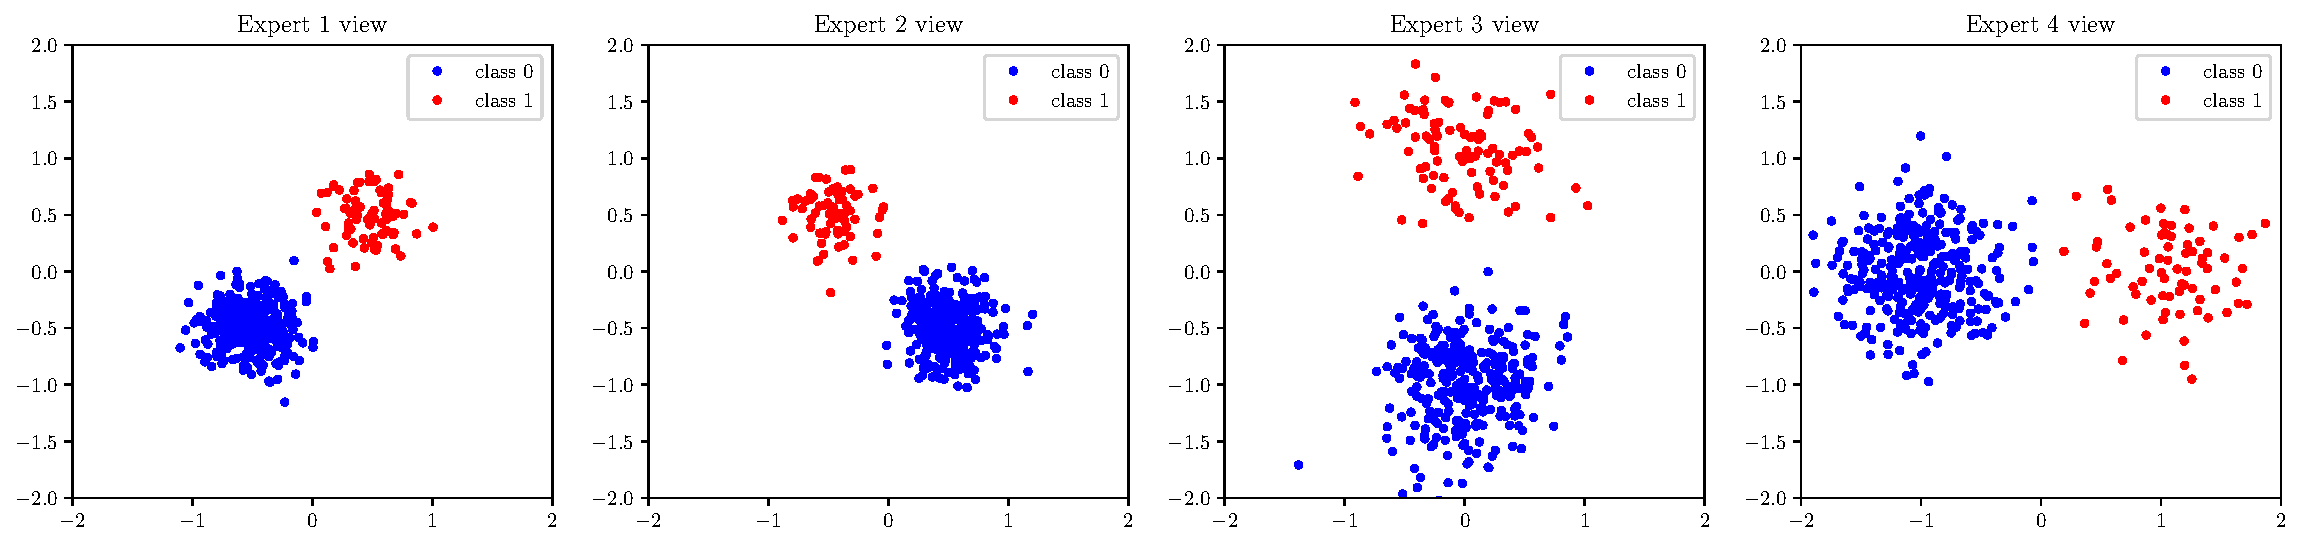
\includegraphics[width=1.0\textwidth]{figures/expert_example}
\caption{Представление объектов разными экспертами}
\label{intro:fig1}
\end{figure}

В отличии от классической постановки смеси экспертов, обучение с экспертом предполагает, что каждая модель имеет собственное признаковое описание объектов, которое построено на основе экспертной информации. Например рассмотрим следующую задачу: пусть объекты это люди, а в качестве экспертов рассмотрим врачей, требуется определить больной человек или нет. На рис.~\ref{intro:fig1} показаны представления о людях разными врачами -- экспертами. Класс~$1$ у каждого эксперта отвечает тому, что человек имеет болезнь по профессии соответствующего врача. Видно, что в пространстве каждого эксперта люди с соответствующей болезнью линейно отделимы от остальных людей с точностью 100\%. Заметим, что если объединить все признаки в одно пространство и построить линейную модель, то получим качество 95\% точности. 

Для оптимизации параметров ансамбля моделей вводится функция ошибки. Она состоит из двух слагаемых: функции регуляризации, вид которой основан на экспертной информации, и ошибки локальных линейных моделей. Качество мультимодели оценивается с помощью интерпретируемого критерия качества.

В вычислительном эксперименте проводиться анализ качества аппроксимации в зависимости от заданных априорных предположений и от уровня шума в данных.

\section{Постановка задачи нахождения параметров кривых второго порядка на изображении}
Задано бинарное изображение. Эксперт предполагает, что на нем изображен конечный набор кривых второго порядка: $$ \mathbf{M} \in \{0, 1 \}^{m_1\times m_2},$$
где 1 отвечает черной точке изображения, а 0~---~белой точке фона. По изображению $\mathbf{M}$ строится выборка $\mathbf{C}$, элементами которой являются координаты $(x_i, y_i)$ черных точек: $$\mathbf{C} \in \mathbb{R}^{N \times 2}.$$
\textbf{Построение признакового описания на основе экспертной информации.} Пусть для набора точек $\mathbf{C} \in \mathbb{R}^{N \times 2}$, образующих кривую $\Omega, $ задано экспертное описание $E(\Omega)$. Множество $E(\Omega)$ состоит из ожидаемого экспертом вида фигуры $\Omega$ и множества ее допустимых преобразований. На основе экспертного описания введем отображения 
\begin{equation}\label{eq1}
K_{x}\bigl(E(\Omega)\bigr): \mathbb{R}^{2} \rightarrow \mathbb{R}^{n}, \quad K_{y}\bigl(E(\Omega)\bigr): \mathbb{R}^{2} \rightarrow \mathbb{R},
\end{equation} 
иными словами, поэлементно:
\begin{equation}\label{eq2}
K_{x}\bigl(E(\Omega\bigr), \mathbf{c}) = \mathbf{x}, \quad  K_{y}\bigl(E(\Omega), \mathbf{c}\bigr) = y
.\end{equation} 
Здесь $n$~---~число признаков, $\mathbf{c} = (x_i, y_i)$~---~точка из выборки $\mathbf{C}$. Рассмотрим линейную модель
\begin{equation}
g: \, \mathbb{R}^n \times \mathbb{R}^n \rightarrow \mathbb{R},
\end{equation}
\begin{equation}\label{eq3}
g(\mathbf{x}, \mathbf{w}) = \mathbf{x}^\mathsf{T} \mathbf{w}.
\end{equation}
Вектор $\hat{\mathbf{w}}= [w_0, \, w_1, \dots, w_n]$ является решением следующей оптимизационной задачи:  \begin{equation} \hat{\mathbf{w}} = \arg\min_{\mathbf{w}\in\mathbb{R}^n} \|g(\mathbf{x}, \mathbf{w}) - y \|, \end{equation} 
Применяя отображения \eqref{eq2} к исходному набору точек $\mathbf{C}$, получим выборку 
\begin{equation}\label{eq4}
    \mathfrak{D} = \{(\mathbf{x}, y) \; | \; \forall \mathbf{c} \in \mathbf{C} \; \mathbf{x} = K_x(\mathbf{c}), \; y = K_y(\mathbf{c}) \}.
    \end{equation} 
    Таким образом, задача определения коэффициентов уравнения исходной фигуры сводится к решению задачи линейной регрессии, т.~е. нахождения компонент вектора $\hat{\mathbf{w}}$, связывающего полученные $\mathbf{x}$ и $y$. \\
\textbf{Мультимодель.} В случае, когда на изображении $K$ кривых второго порядка  $\Omega_1, \dots, \Omega_K$, для каждой из которых имеется экспертная информация $E_k = E(\Omega_k), \, k \in \{1, \dots, K\}$, ставится задача построения мультимодели, называемой смесью $K$ экспертов. 
\begin{definition} Назовем мультимодель $f$ смесью K экспертов \begin{equation}
  f = \sum\limits_{k = 1}^{K}\pi_k(\mathbf{x}, \mathbf{V})g_k(\mathbf{w}_k),  \; \; \; \; \pi_k(\mathbf{x}, \mathbf{V}): \mathbb{R}^{2\times |\mathbf{V}|} \rightarrow [0, \, 1], \; \; \; \; \sum\limits_{k = 1}^{K}\pi_k(\mathbf{x}, \mathbf{V}) = 1, 
\end{equation} где $g_k$~---~локальная модель, называемая экспертом, $\mathbf{x}$~---~признаковое описание объекта, $\pi_k$~---~шлюзовая функция, вектор $\mathbf{w}_k$~---~параметры локальной модели, вектор $\mathbf{V}$~---~параметры шлюзовой функции. В данной работе $g_k$~---~линейная модель. \end{definition}

Для каждой кривой второго порядка заданы отображения (\ref{eq1}). Тогда, используя локальные линейные модели, построим универсальную мультимодель, описывающую все множество кривых $\Omega_1, \dots, \Omega_K$ на изображении $\mathbf{M}$:
\begin{equation}\label{5}
f = \sum\limits_{(\mathbf{x}, y) \in \mathfrak{D}} \sum\limits_{k = 1}^{K} \pi_k(\mathbf{x}, \mathbf{V})g_k(\mathbf{x}, \mathbf{w}_k), 
\end{equation} где $\pi_k$~---~шлюзовая функция: 
\begin{equation}\label{6}
\pi_k(\mathbf{x}, \mathbf{V}): \mathbb{R}^{2\times |\mathbf{V}|} \rightarrow [0, \, 1], \; \; \; \; \sum\limits_{k = 1}^{K}\pi_k(\mathbf{x}, \mathbf{V}) = 1,\end{equation}
    $\mathbf{V}$~---~параметры шлюзовой функции, а $g_k$~---~локальная линейная модель вида (\ref{eq3}).
    
В данной работе
\begin{equation}
    \boldsymbol{\pi}(\mathbf{x}, \mathbf{V}) = \text{softmax}\bigl(\mathbf{V}_1^{\mathsf{T}}\boldsymbol{\sigma}(\mathbf{V}_2^{\mathsf{T}}\mathbf{x}) \bigr),
\end{equation}
где $\mathbf{V} = \{ \mathbf{V}_1, \, \mathbf{V}_2\}$~---~параметры шлюзовой функции, $\mathbf{V}_1 \in \mathbb{R}^{p \times k}, \, \mathbf{V}_2 \in \mathbb{R}^{n \times p}$. 

Для нахождения оптимальных параметров мультимодели необходимо решить следующую задачу оптимизации:
\begin{equation}\label{9}
\mathcal{L} = \sum\limits_{(\mathbf{x}, y) \in \mathfrak{D}} \sum\limits_{k = 1}^{K} \pi_k(\mathbf{x}, \mathbf{V})(y - \mathbf{w}_k^{\mathsf{T}}\mathbf{x})^2 + R\bigl(\mathbf{V}, \mathbf{W}, E(\Omega)\bigr) \rightarrow \min_{\mathbf{V}, \mathbf{W}},
\end{equation}
где $\mathbf{W} = [\mathbf{w}_1, \dots, \mathbf{w}_k]$~--- параметры локальных моделей, $R\bigl(\mathbf{V}, \mathbf{W}, E(\Omega)\bigr)$~---~регуляризация параметров, основанная на экспертной информации.

\section{Построение признакового описания фигур}
\paragraph{Окружность.}
Пусть $(x_0, y_0)$~---~центр окружности, которую необходимо найти на бинарном изображении $\mathbf{M}$, а $r$~---~ее радиус. Элементы выборки $(x_i, y_i) \in \mathbf{C}$ являются геометрическим местом точек, которое аппроксимируется уравнением окружности:
\begin{equation}
(x_i - x_0)^2 + (y_i - y_0)^2 = r^2.
\end{equation}
Раскрыв скобки, получим:
\begin{equation}(2x_0)\cdot x_i + (2y_0)\cdot y_i + (r^2 - x_0^2 - y_0^2)\cdot 1 = x_i^2 + y_i^2 . 
\end{equation}
Тогда отображения (\ref{eq2}) примут вид:
\begin{equation}
\label{10}
K_{x}(\mathbf{c}_i) = [x_i, \, y_i, \, 1] = \mathbf{x}, \,  K_{y}(\mathbf{c}_i) = x_i^2+y_i^2 = y.
\end{equation} 
Поставим задачу линейной регрессии \eqref{eq4}.
Компоненты вектора $\mathbf{w} = [w_0, \, w_1, \, w_2]^\mathsf{T}$, связывающего $\mathbf{x}$ и $y$, восстанавливают параметры окружности: \begin{equation} x_0 = \frac{w_0}{2}, \; y_0 = \frac{w_1}{2}, \; r = \sqrt{w_3 + x_0^2 + y_0 ^2}.\end{equation}
\paragraph{Эллипс.} Элементы выборки $(x_i, y_i) \in \mathbf{C}$ являются ГМТ, которое аппроксимируется уравнением общим уравнением эллипса: 
\begin{equation}
Ax_i^2+Bx_iy_i+Cy_i^2 + Dx_i + Ey_i + F = 0, \qquad B^2 - 4AC < 0.
\end{equation}
Из условия на коэффициенты $A, \, B, \, C$ следует, что $A \neq 0, \, C \neq 0$. 
Перепишем уравнение:
\begin{equation}
B'x_iy_i + C'y_i^2 + D'x_i + E'y_i + F' = x_i^2.
\end{equation}
В этом случае отображения (\ref{eq2}) имеют вид: 
\begin{equation}
K_{x}(\mathbf{c}_i) = [x_iy_i, \, y_i^2, \, x_i, \, y_i, \, 1] = \mathbf{x}, \,  K_{y}(\mathbf{c}_i) = x_i^2 = y.
\end{equation}
Поставим задачу линейной регрессии \eqref{eq4}.
Оптимальные параметры линейной регрессии и коэффициенты уравнения связаны следующим образом: \begin{equation}w_0 = B' = -\frac{B}{A}, \, w_1 = C' = -\frac{C}{A}, \, w_2 = D' = -\frac{D}{A}, \, w_3 = E' = -\frac{E}{A}, \, w_4 = F' = -\frac{F}{A},\end{equation} с учетом \begin{equation} \label{16}B^2 - 4AC < 0,\end{equation} то есть
\begin{equation}
\label{3.10}
w_0^2 + 4w_1 < 0.
\end{equation}

\paragraph{Парабола.} Элементы выборки $\mathbf{C}$ аппроксимируются общим уравнением параболы: 
\begin{equation} 
\label{24}
Ax_i^2 + Bx_iy_i + Cy_i^2 + Dx_i + Ey_i + F = 0, \qquad B^2 = 4AC.
\end{equation} где 
Рассмотрим различные варианты расположения параболы относительно координатных осей. \\
В случае, если ось симметрии параболы параллельна $Ox$, из экспертных данных следует, что коэффициенты общего уравнения параболы 
\begin{equation}
\label{25}
A = B = 0.
\end{equation}
Тогда общее уравнение параболы, аппроксимирующее выборку $\mathbf{C}$, приобретает вид \begin{equation}Cy_i^2 + Dx_i + Ey_i + F = 0 .\end{equation}
Перепишем: \begin{equation}y_i^2 = D'x_i + E'y_i + F'.\end{equation}
Тогда вид преобразований (\ref{eq2}): \begin{equation}K_{x}(\mathbf{c}_i) = [x_i, y_i, 1] = \mathbf{x}, \,  K_{y}(\mathbf{c}_i) = y_i^2 = y. \end{equation} 
Поставим задачу линейной регрессии \eqref{eq4}.
Параметры параболы выражаются через оптимальные параметры линейной регрессии: \begin{equation} w_0 = D' = -\frac{D}{C}, \,  w_1 = E' = -\frac{E}{C}, \,  w_2 = F' = -\frac{F}{C}.\end{equation}
В случае, если ось симметрии параболы параллельна $Oy$, то аналогично предыдущему случаю, общее уравнение приобретет вид: \begin{equation} x_i^2  = D'x_i + E'y_i + F'.\end{equation}
Преобразования (\ref{eq2}) будут иметь вид: \begin{equation}K_{x}(\mathbf{c}_i) = [x_i, y_i, 1] = \mathbf{x}, \,  K_{y}(\mathbf{c}_i) = x_i^2 = y. \end{equation}
В случае, если ось симметрии параболы не параллельна ни одной из координатных осей, то в таком случае $A \neq 0, \, B \neq 0, \, C \neq 0$. \\
Тогда общее уравнение параболы, аппроксимирующее выборку, имеет вид: \begin{equation} x_i^2 = B'x_iy_i + C'y_i^2 + D'x_i + E'y_i + F'.\end{equation}
Преобразования (\ref{eq2}): \begin{equation} K_{x}(\mathbf{c}_i) = [x_iy_i, \, y_i^2, \, x_i, \, y_i, \, 1] = \mathbf{x}, \,  K_{y}(\mathbf{c}_i) = x_i^2 = y.\end{equation}
Поставим задачу линейной регрессии \eqref{eq4}.
Исходные параметры параболы восстанавливаются по вектору оптимальных параметров линейной регрессии $\mathbf{w}$следующим образом: \begin{equation} w_0 = B' = -\frac{B}{A}, \, w_1 = C' = -\frac{C}{A}, \, w_2 = D' = -\frac{D}{A}, \, w_3 = E' = -\frac{E}{A}, \, w_4 = F' = -\frac{F}{A}.\end{equation}
\paragraph{Гипербола.}
Элементы выборки $\mathbf{C}$ аппроксимируются общим уравнением гиперболы: \begin{equation} Ax_i^2 + Bx_iy_i + Cy_i^2 + Dx_i + Ey_i + F = 0,\end{equation} где \begin{equation} \label{35}
B^2 - 4AC > 0.\end{equation} \\
В случае, если полуоси гиперболы параллельны осям координат, то уравнение гиперболы имеет вид: \begin{equation}  Ax_i^2 + Cy_i^2 + Dx_i + Ey_i + F = 0,\end{equation} где \begin{equation} \label{37}
AC < 0.\end{equation} Перепишем уравнение: \begin{equation}
C'y_i^2 + D'x_i + E'y_i + F' = x_i^2.\end{equation} Преобразования (\ref{eq2}): \begin{equation}
K_{x}(\mathbf{c}_i) = [y_i^2, x_i, y_i, 1] = \mathbf{x}, \,  K_{y}(\mathbf{c}_i) = x_i^2 = y.\end{equation} \\
В случае, если полуоси гиперболы непараллельны осям координат, то $B \neq 0$. Перепишем уравнение гиперболы:\begin{equation}A'x_i^2 + C'y_i^2 + D'x_i + E'y_i + F' =  x_iy_i.\end{equation} Преобразования (\ref{eq2}): \begin{equation}
K_{x}(\mathbf{c}_i) = [x_i^2, y_i^2, x_i, y_i, 1] = \mathbf{x}, \,  K_{y}(\mathbf{c}_i) = x_iy_i = y.\end{equation} 

\paragraph{Единое пространство для кривых второго порядка.} Произвольная кривая второго порядка, главная ось которой не параллельна оси ординат задается следующим выражением:
\[
\label{st:coef}
x^2 = B'xy+C'y^2+D'x+E'y+F',
\]
где на коэффициенты $B',C'$ накладываются ограничения, которые зависят от вида кривой. Выражение~\eqref{eq2} принимает следующий вид:
\[
\label{st:K_map}
K_x\bigr(\mathbf{c}_i\bigr)=\left[x_iy_i, y_i^2, x_i, y_i, 1\right], \quad K_y\bigr(\mathbf{c}_i\bigr)=x_i^2,
\]
откуда получаем задачу линейной регрессии для восстановления параметров~$B', C', D', E', F'$ по составленной выборке.

\section{Композиция фигур}
Для построения композиции фигур воспользуемся выражением~\eqref{9} принимает следующий вид:
\begin{equation} 
\label{statment:optim:task}
\begin{aligned}
\mathcal{L} = \sum\limits_{\mathbf{c} \in \mathbf{C}} \sum\limits_{k = 1}^{K} \pi_k(\mathbf{c}, \mathbf{V})\left(K^{k}_y\bigr(\mathbf{c}\bigr) - \mathbf{w}_k^{\mathsf{T}}K^{k}_x\bigr(\mathbf{c}\bigr)\right)^2 + R\bigl(\mathbf{V}, \mathbf{W}, E(\Omega)\bigr) \rightarrow \min_{\mathbf{V}, \mathbf{W}},
\end{aligned}
\end{equation} 
где~$K^{k}_x, K^{k}_y$ экспертное представление~$k$-го эксперта. В качестве регуляризатора~$R$ рассматриваются дополнительные ограничения на вектора параметров моделей: априорное распределение параметров~$\mathbf{w}_1, \cdots \mathbf{w}_k$, а также связь между параметрами вида~\eqref{3.10}. Для решения оптимизационной задачи~\eqref{statment:optim:task} предлагается использовать EM--алгоритм.

\section{Вычислительный эксперимент}
Проведен вычислительный эксперимент для анализа качества моделей кривых второго порядка на изображении. Эксперимент разделе на несколько частей. В первой части проводится анализ сходимости метода в случае, когда задана единственная кривая. Во второй части проводится эксперимент с несколькими окружностями на изображении. В третий части проводится анализ сходимости метода в зависимости от уровня шума в данных и от априорных предположений.

\subsection{Визуализация обучения в случае одной фигуры}
\begin{figure}
\begin{minipage}{.25\textwidth}
      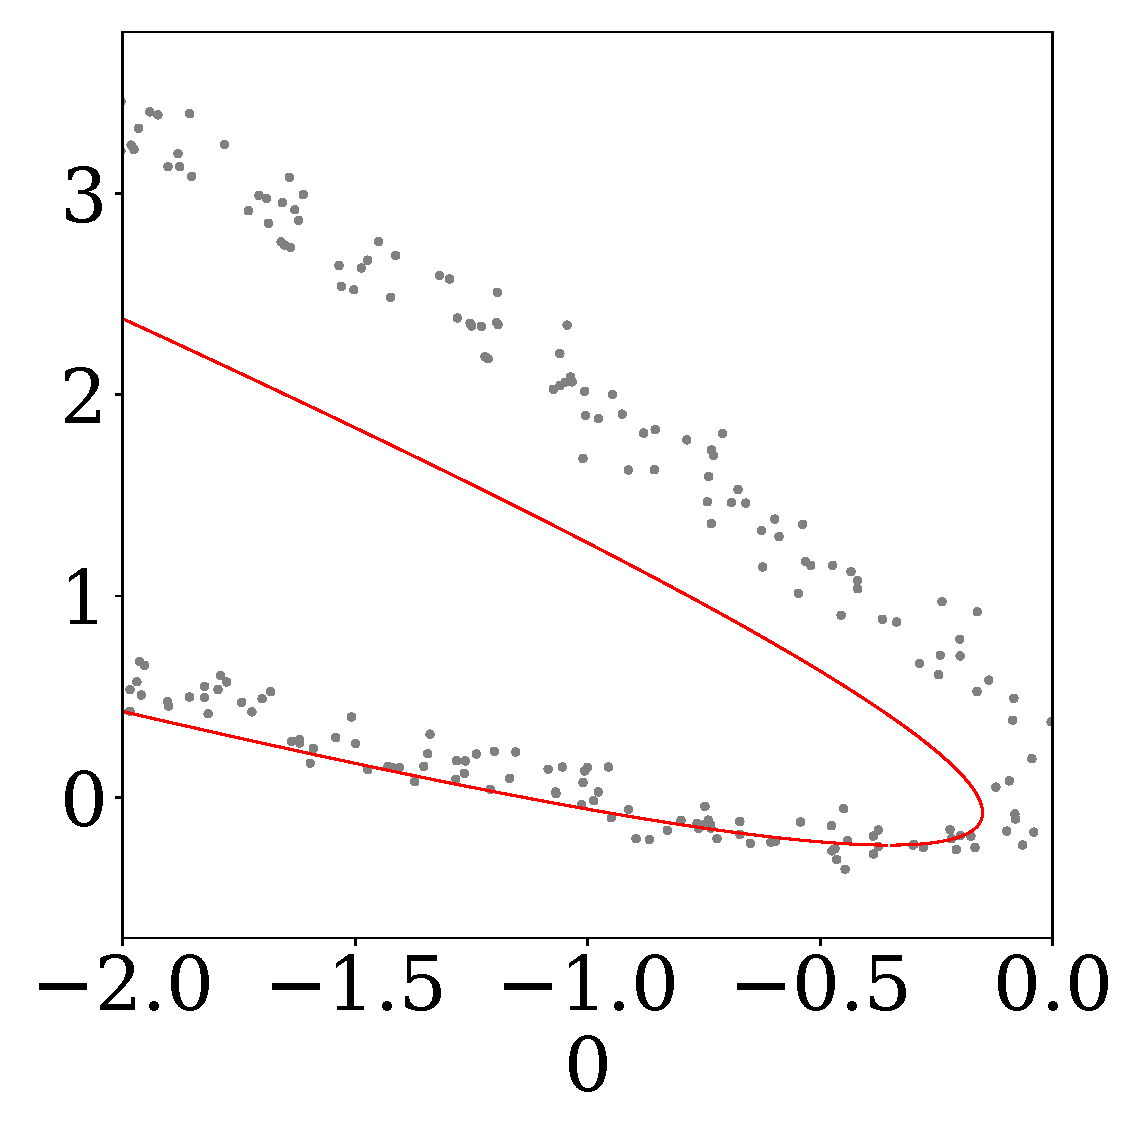
\includegraphics[scale = 0.19]{figures/511_0}
\end{minipage}
\begin{minipage}{.25\textwidth}

      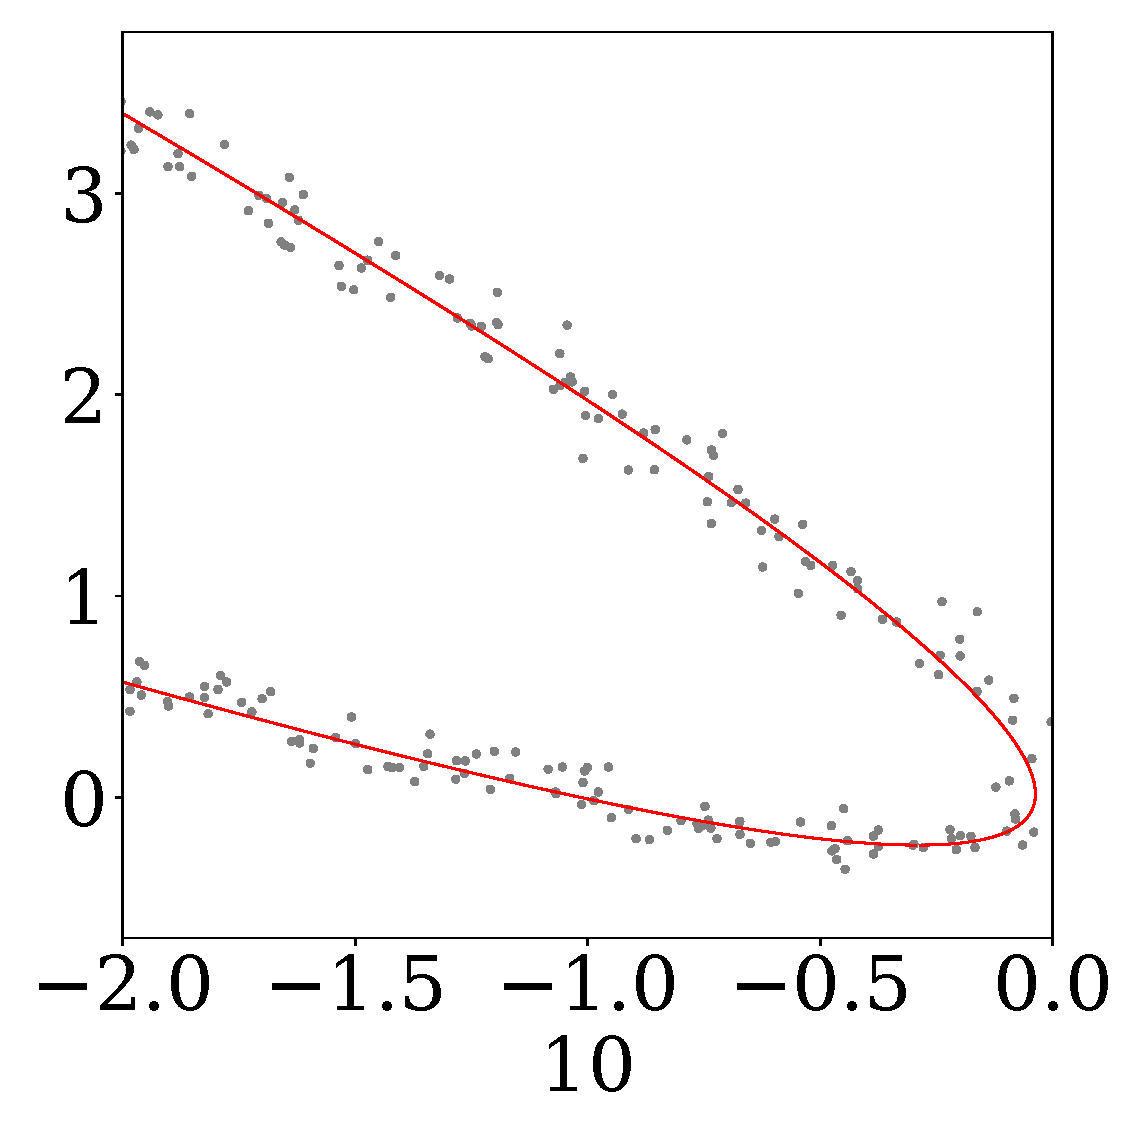
\includegraphics[scale = 0.19]{figures/511_10}
\end{minipage}
\begin{minipage}{.25\textwidth}

      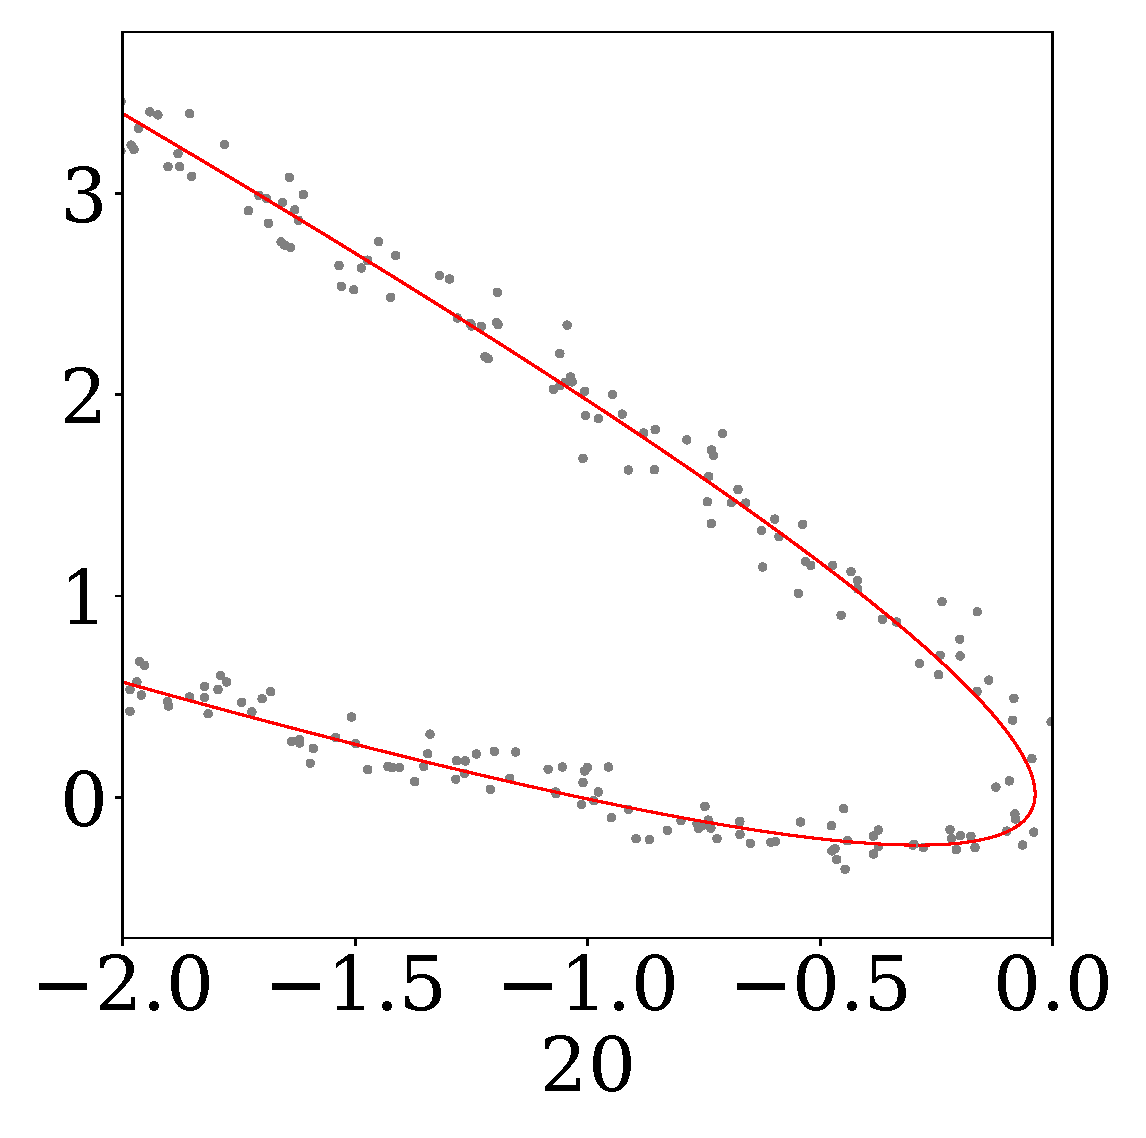
\includegraphics[scale = 0.19]{figures/511_20}
\end{minipage}
\begin{minipage}{.20\textwidth}

      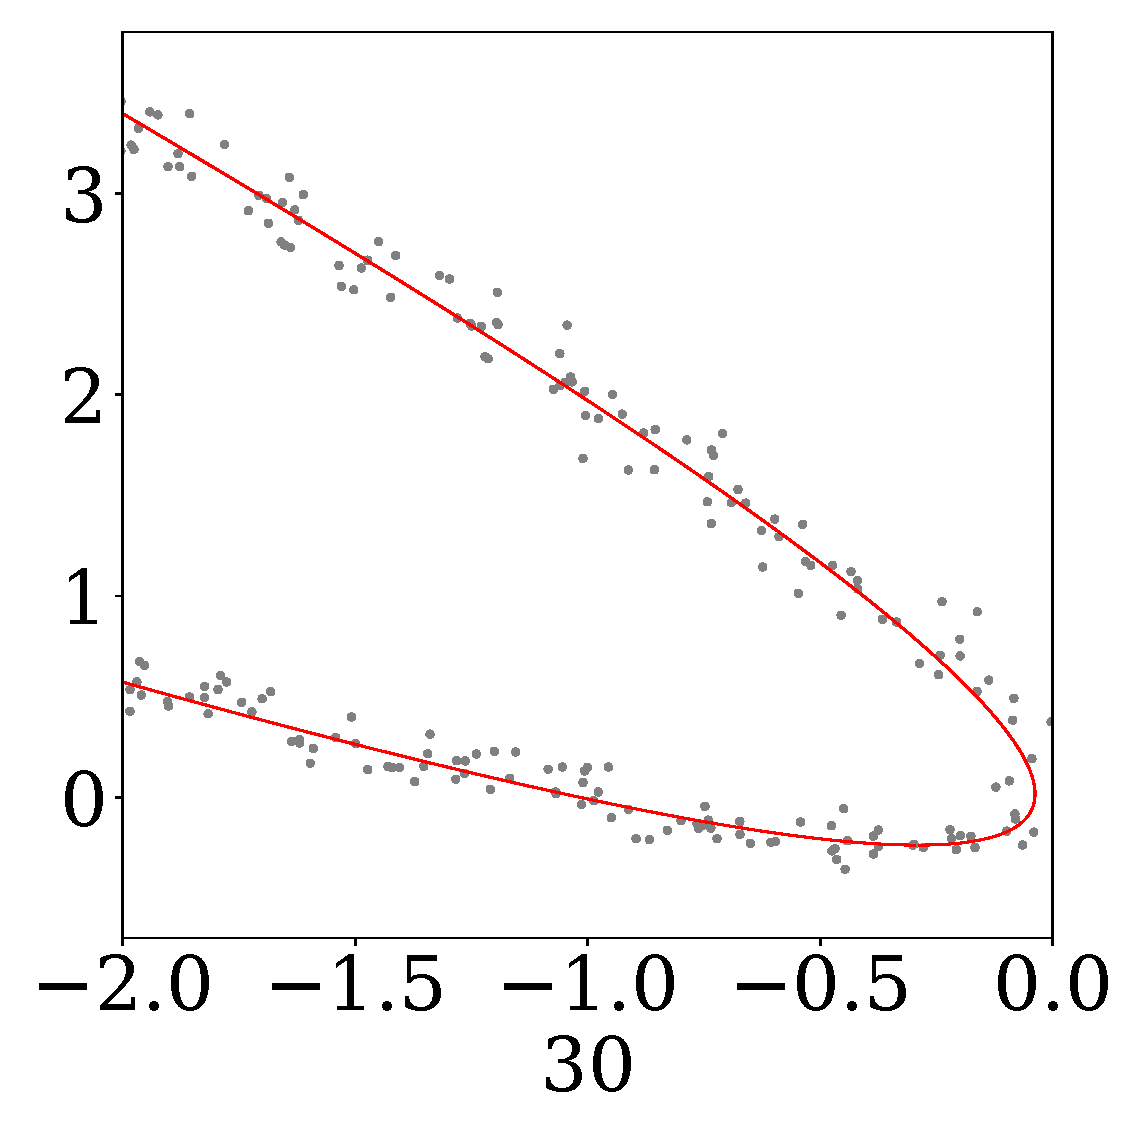
\includegraphics[scale = 0.19]{figures/511_30}
\end{minipage}
\caption{Визуализация процесса обучения в течение 30 итераций.}
\label{ce:fig1}
\end{figure}

\begin{figure}[h!t]\center
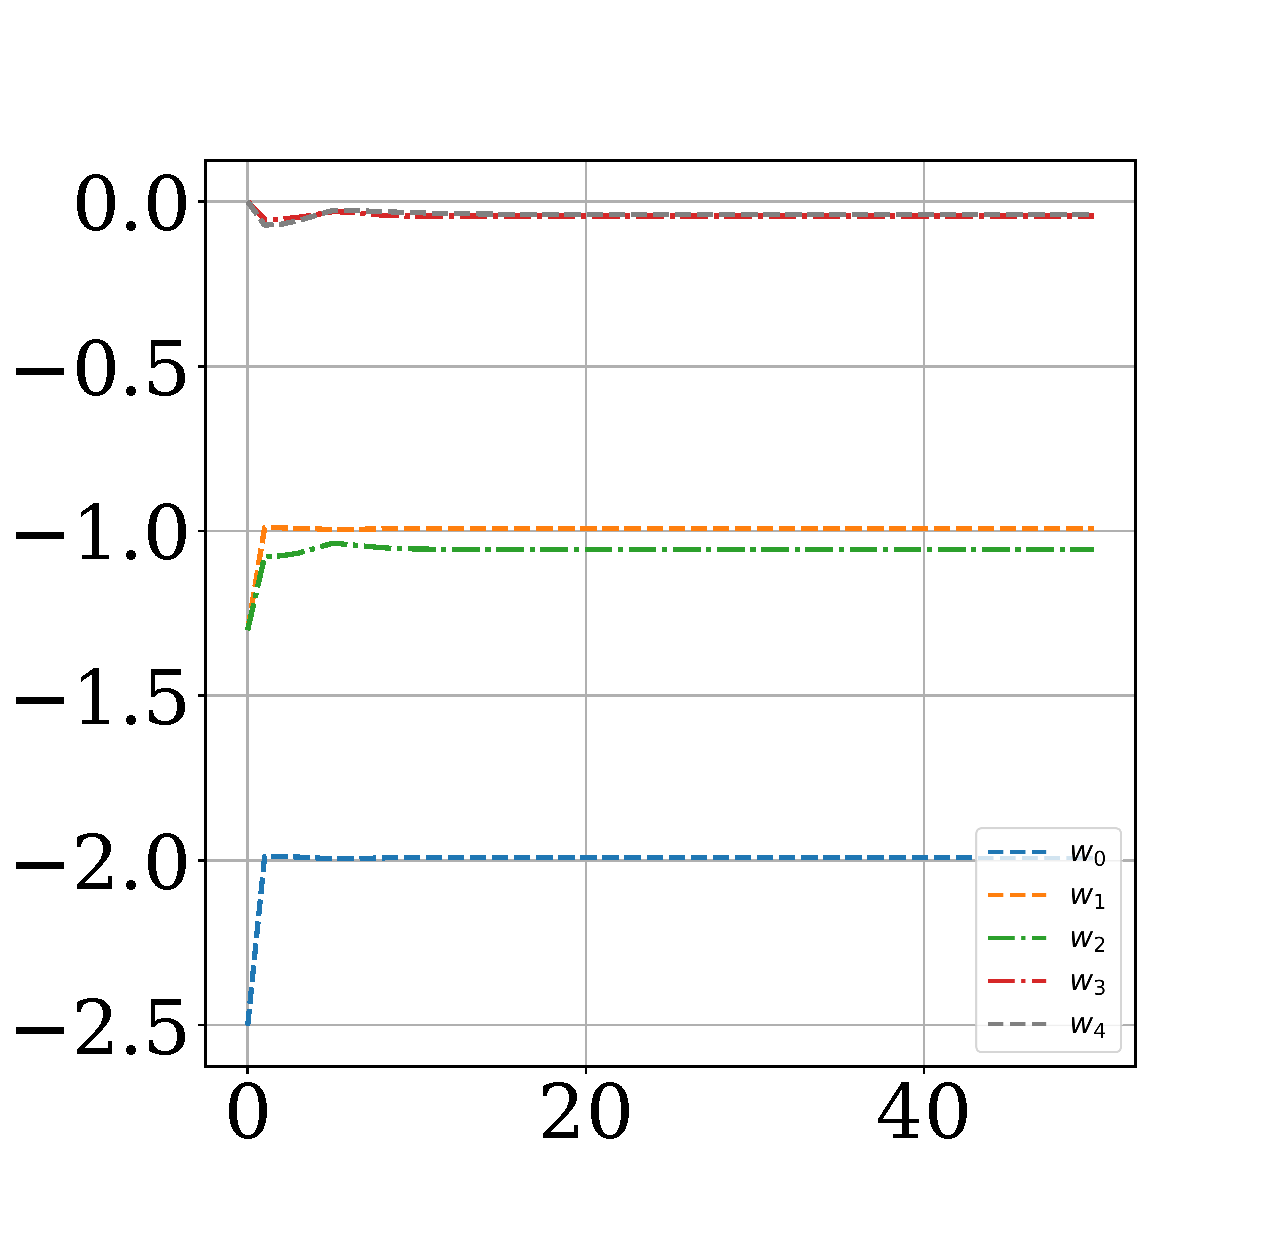
\includegraphics[width=0.5\textwidth]{figures/511w}
\caption{График зависимости $w_i$от номера итерации}
\label{ce:fig2}
\end{figure}

В данной части эксперимента показан пример обучения метода модели линейной регрессии для аппроксимации кривой второго порядка. В качестве данных используется синтетическая выборка Synthetic~1, которая получена при помощи генерации произвольной параболы, главная ось которой не является параллельной оси ординат, а также добавления к точкам нормального шума со средним~$\mu=0$ и дисперсией~$\beta=0{,}1$. В качестве априорных данных задан истинный вектор параметров с нормальным шумом. В данном случае решалась оптимизационая задача~\eqref{statment:optim:task} при количестве локальных моделей~$K=1$ и без регуляризатора~$R=0$.

На рис.~\ref{ce:fig1} показан процесс обучения на выборке Synthetic~1 в течение 30 итераций. Из рисунка видно, что на 10-й итерации модель аппроксимирует выборку с высокой точностью и при дальнейших итерациях качество не изменяется. На рис.~\ref{ce:fig2} показана зависимость значения параметров от номера итерации. Видно, что после малого количества итераций 


\subsection{Эксперимент с окружностями}
\begin{figure}[h!]
\begin{minipage}{.32\textwidth}
      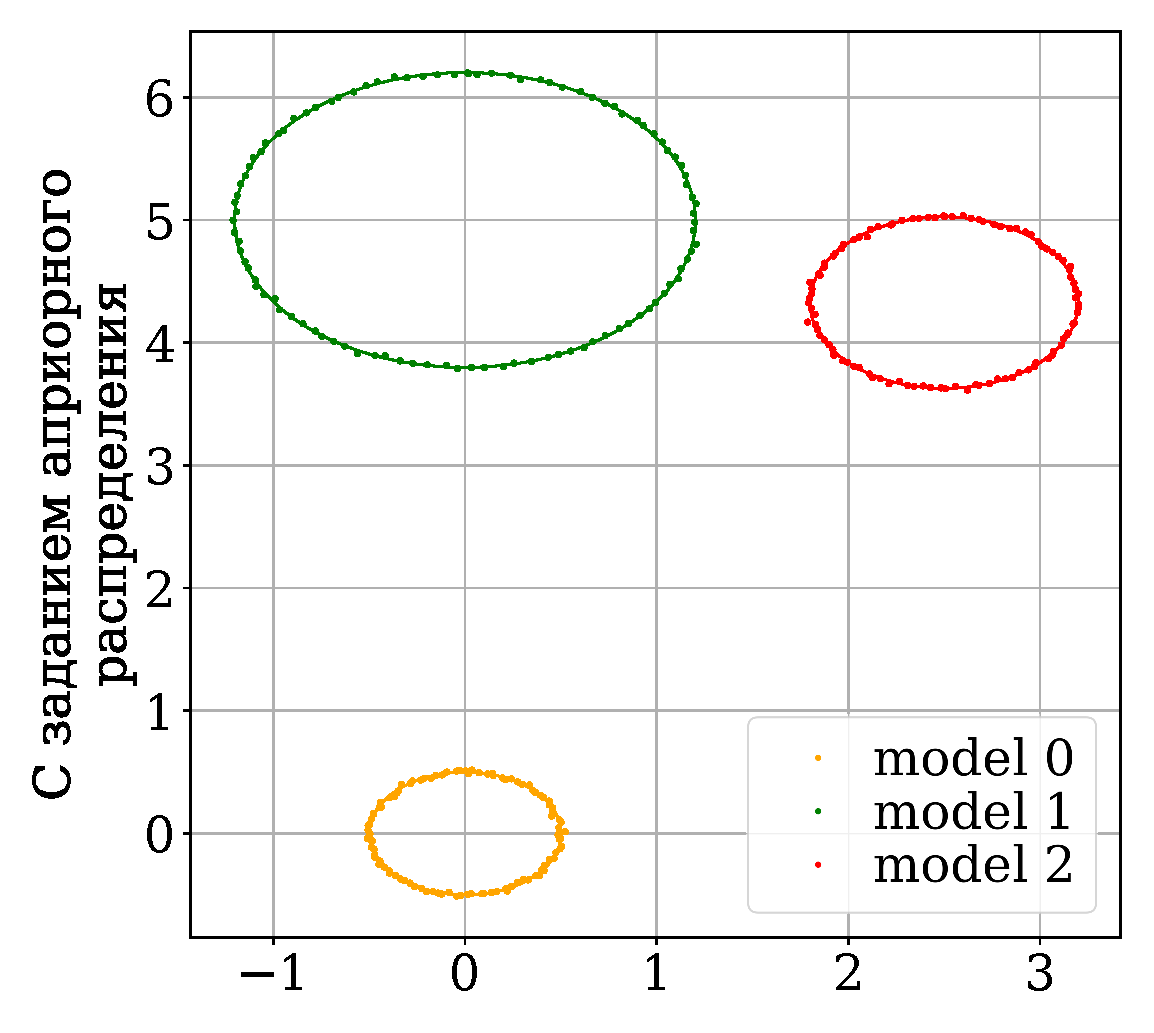
\includegraphics[width =  \textwidth]{figures/910.eps}
\end{minipage}
\begin{minipage}{.32\textwidth}
\hspace{0.3mm}
      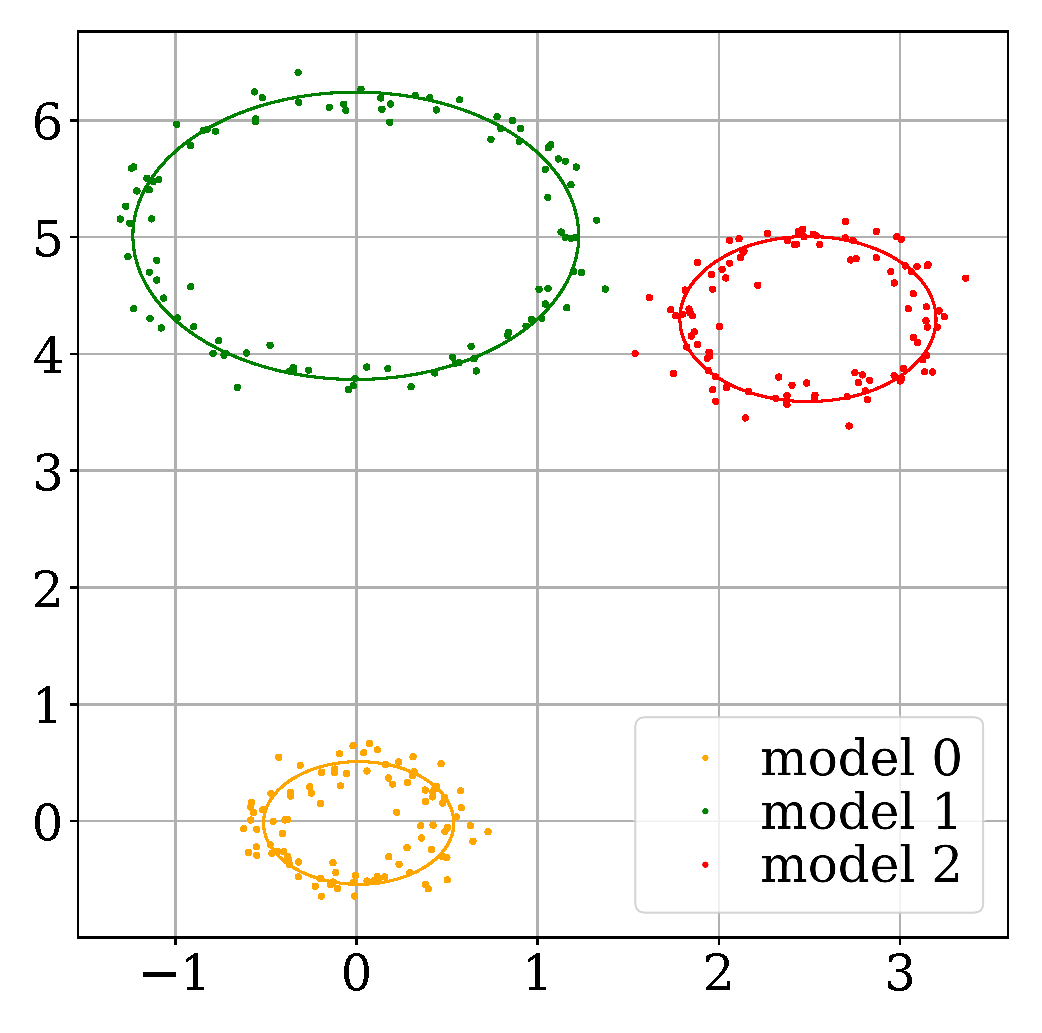
\includegraphics[width =  0.89\textwidth]{figures/901.eps}
\end{minipage}
\begin{minipage}{.32\textwidth}
\vspace{-3mm}
\hspace{-8.5mm}
      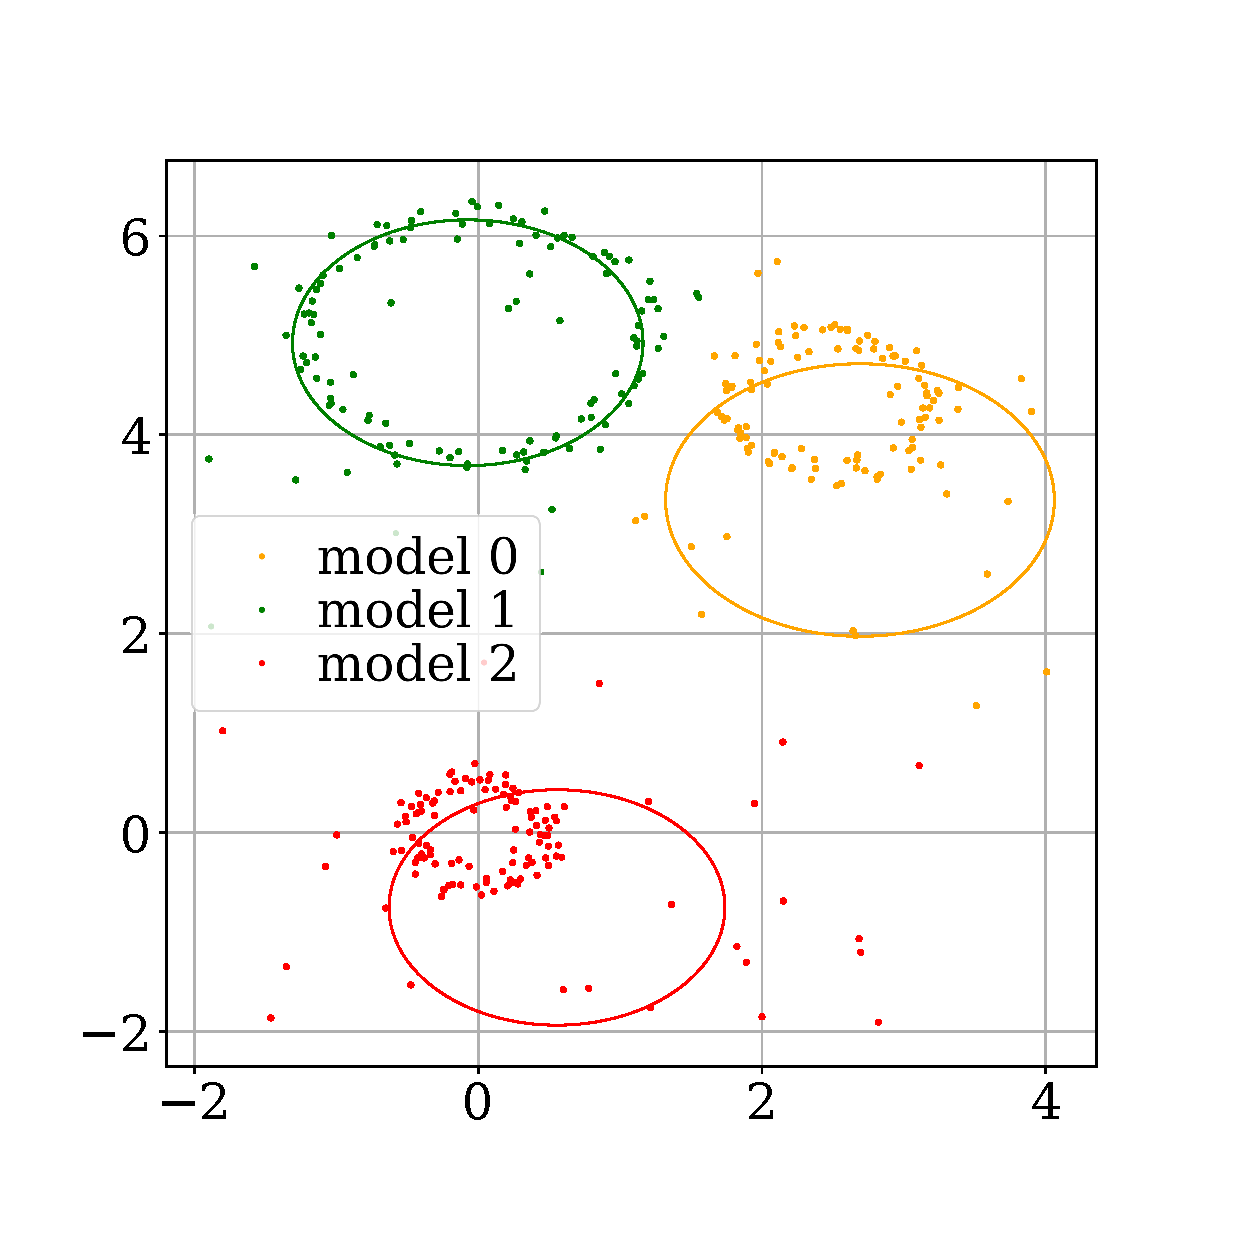
\includegraphics[width =  1.07\textwidth]{figures/902.eps}
\end{minipage}
\begin{minipage}{.32\textwidth}
      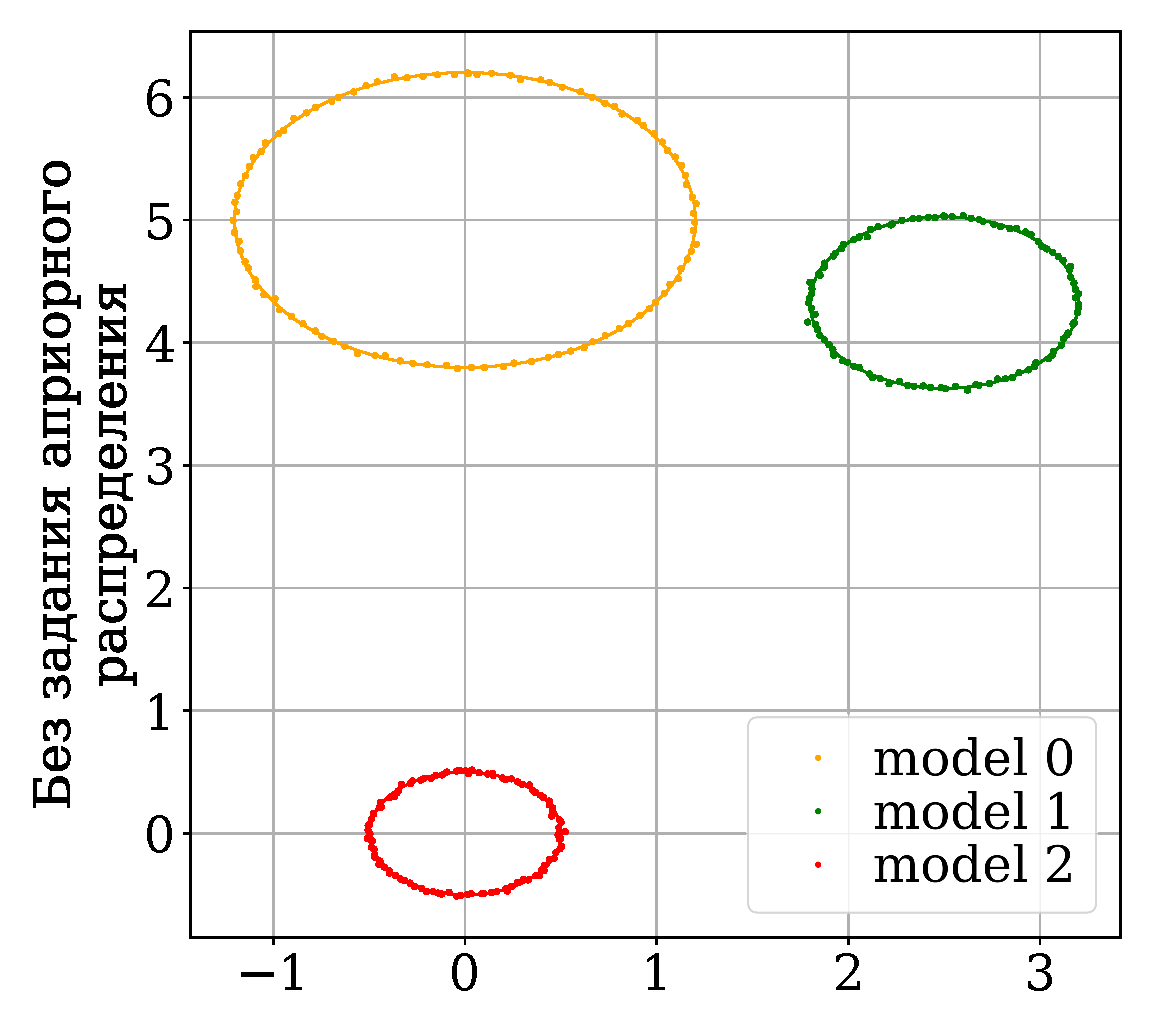
\includegraphics[width =  \textwidth]{figures/900.eps}
\end{minipage}
\begin{minipage}{.32\textwidth}
\hspace{2mm}
      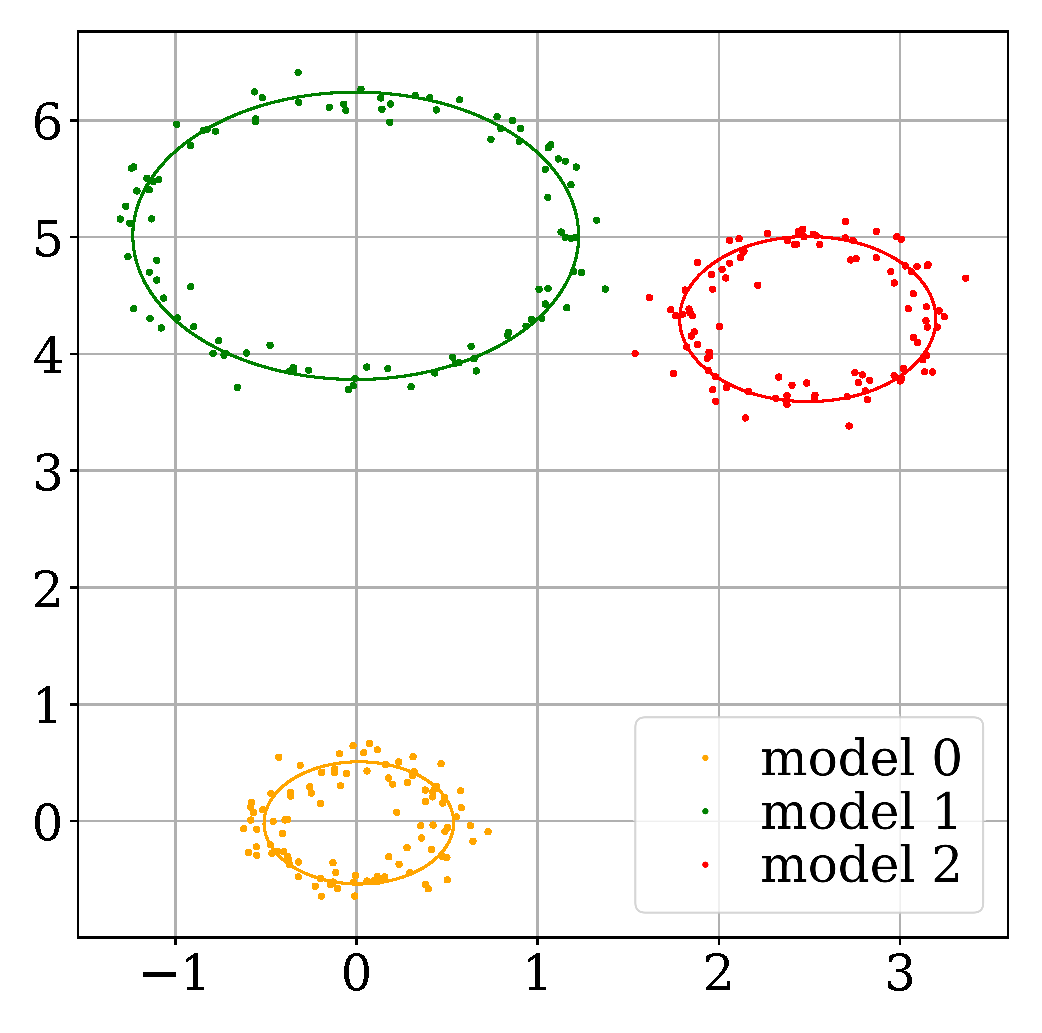
\includegraphics[width =  0.9\textwidth]{figures/911.eps}
\end{minipage}
\begin{minipage}{.32\textwidth}
\hspace{-2.3mm}
      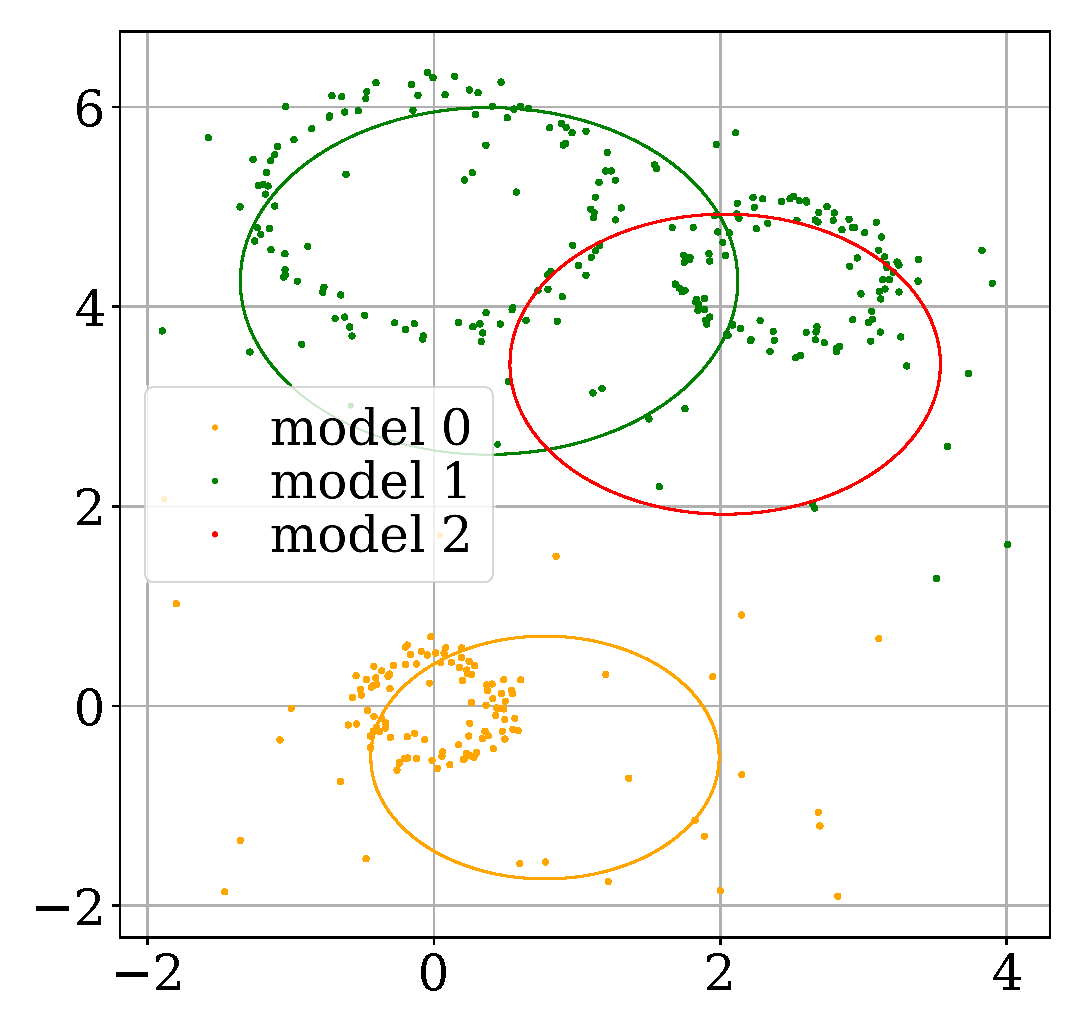
\includegraphics[width =  0.935\textwidth]{figures/912.eps}
\end{minipage}
\caption{Мультимодель в зависимости от разных априорных предположений и уровня шума. Сверху вниз: построение с заданием априорного распределения; без задания априорного распределения. Слева на право: окружности без шума; шум в радиусе окружности; шум в радиусе окружности а также произвольные точки по всему изображению.}
\label{ce:fig3}
\end{figure}

\begin{figure}[h]
\begin{minipage}{.32\textwidth}
\hspace{-3mm}
      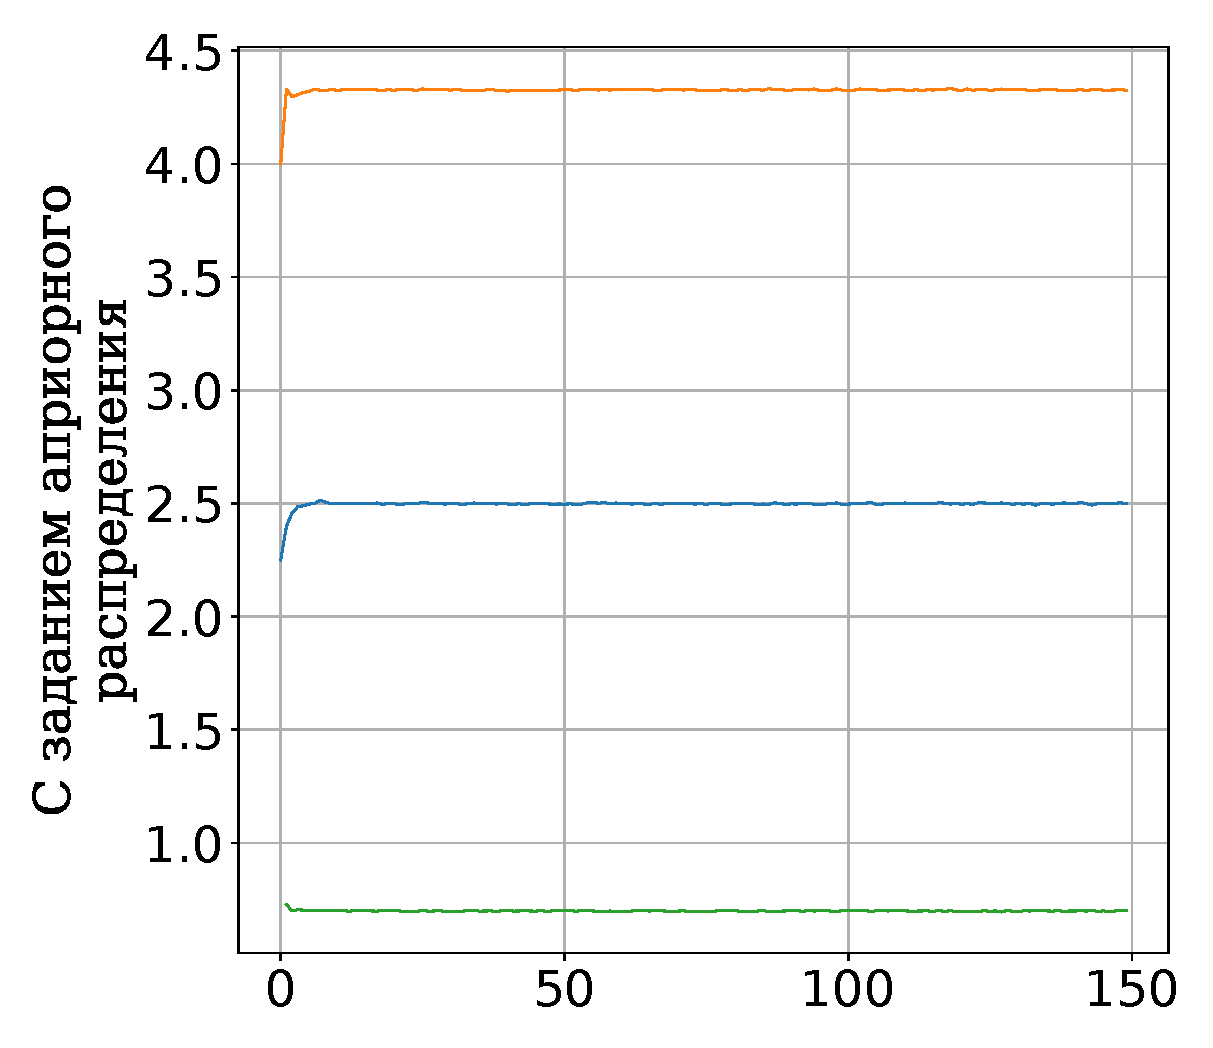
\includegraphics[width = 1.05\textwidth]{figures/910noise.eps}
\end{minipage}
\begin{minipage}{.32\textwidth}
\vspace{2pt}
\hspace{-2.1mm}
      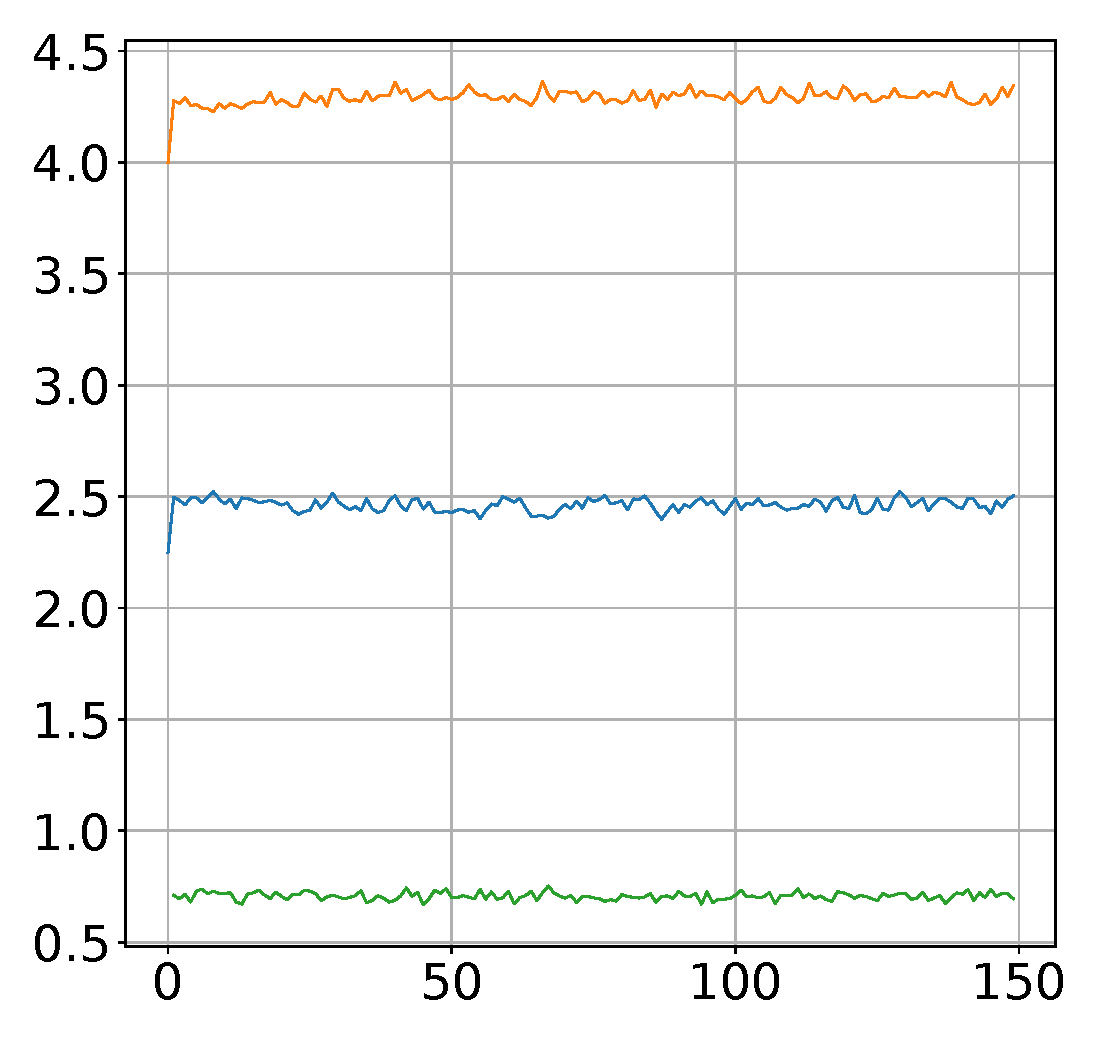
\includegraphics[width = 0.95\textwidth]{figures/911noise.eps}
\end{minipage}
\begin{minipage}{.32\textwidth}
\vspace{2pt}
\hspace{-6.3mm}
      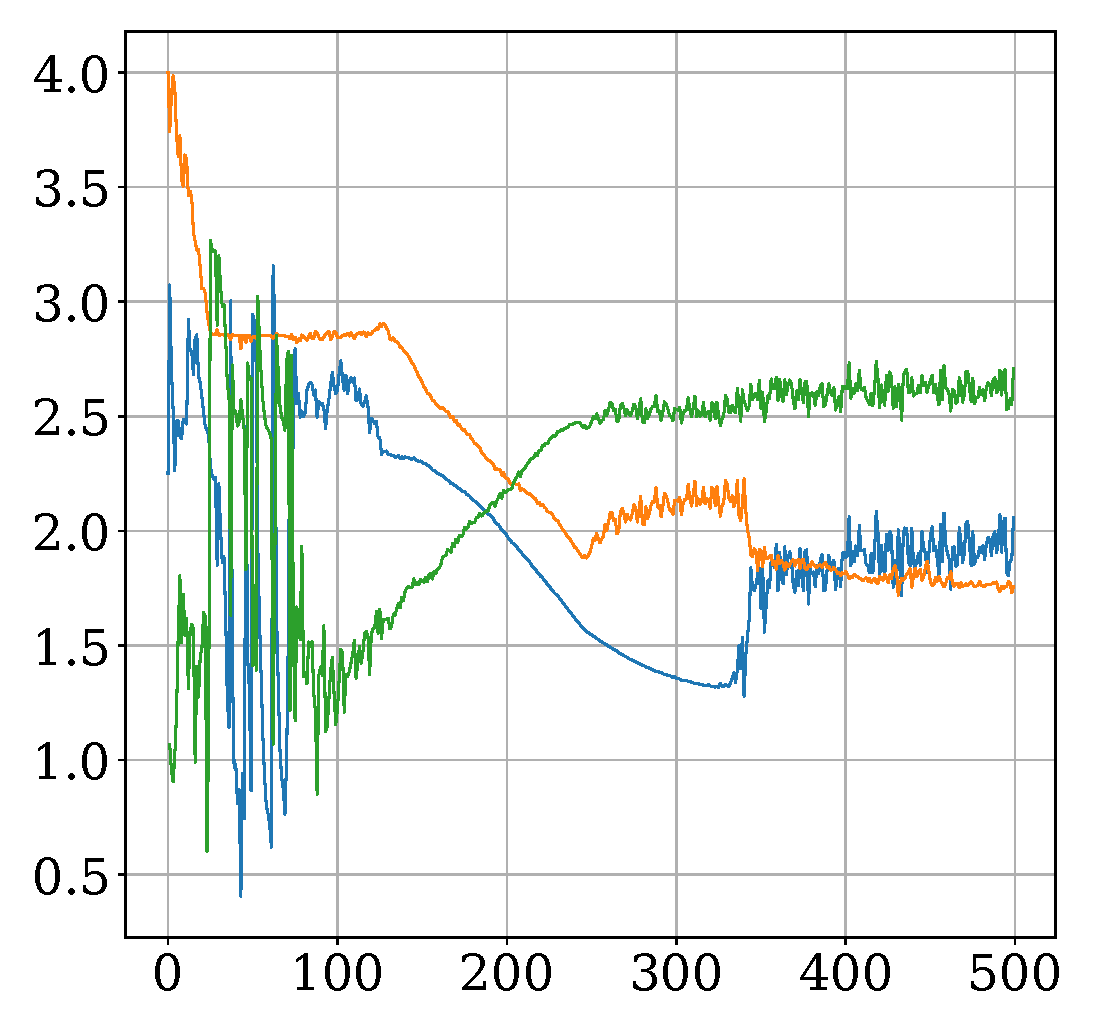
\includegraphics[width = 0.95\textwidth]{figures/912noise.eps}
\end{minipage}
\begin{minipage}{.32\textwidth}
\hspace{-3mm}
      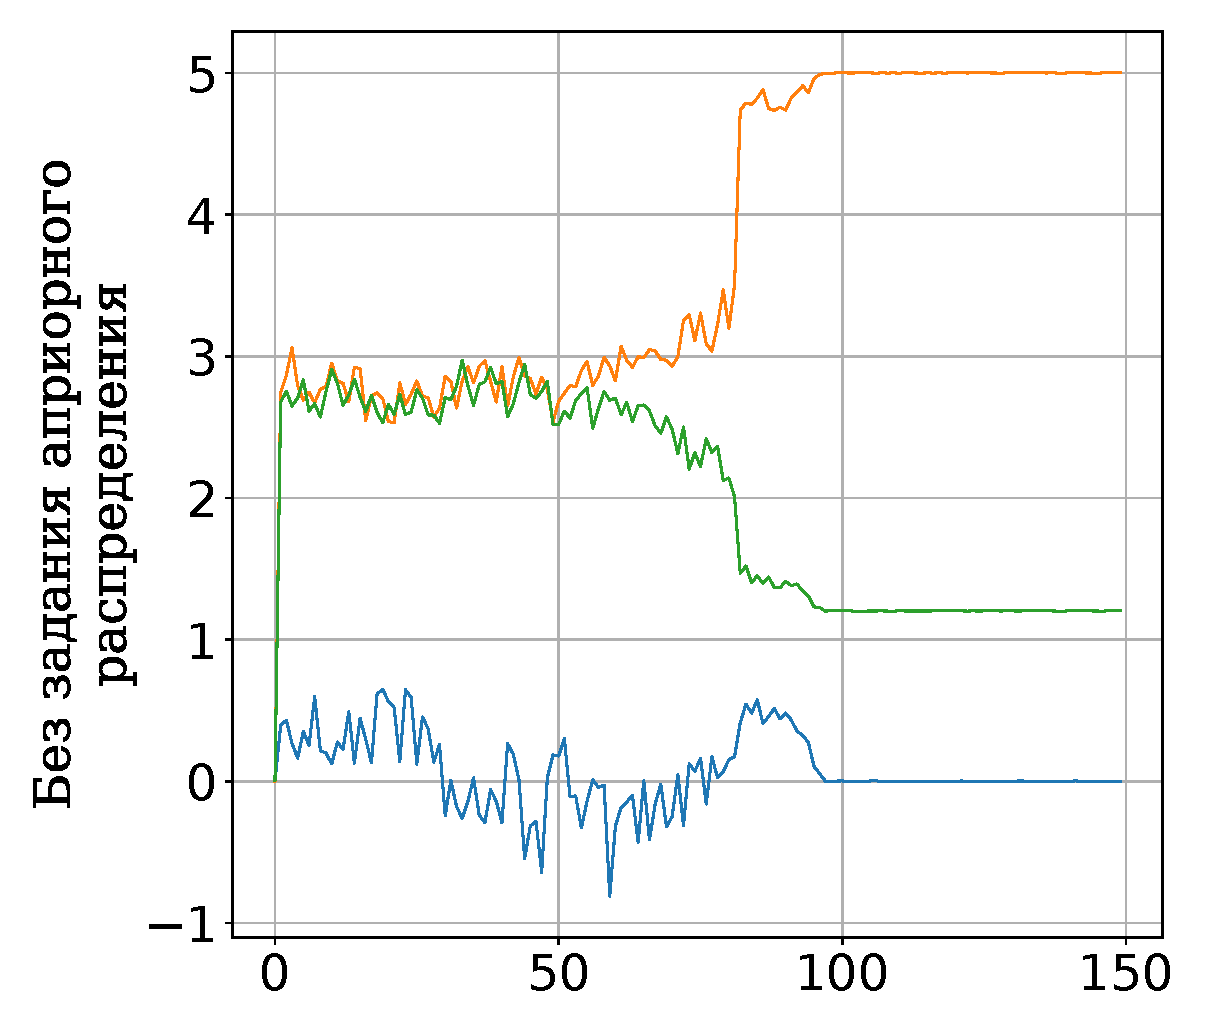
\includegraphics[width = 1.05\textwidth]{figures/900noise.eps}
\end{minipage}
\begin{minipage}{.32\textwidth}
\hspace{-2.1mm}
      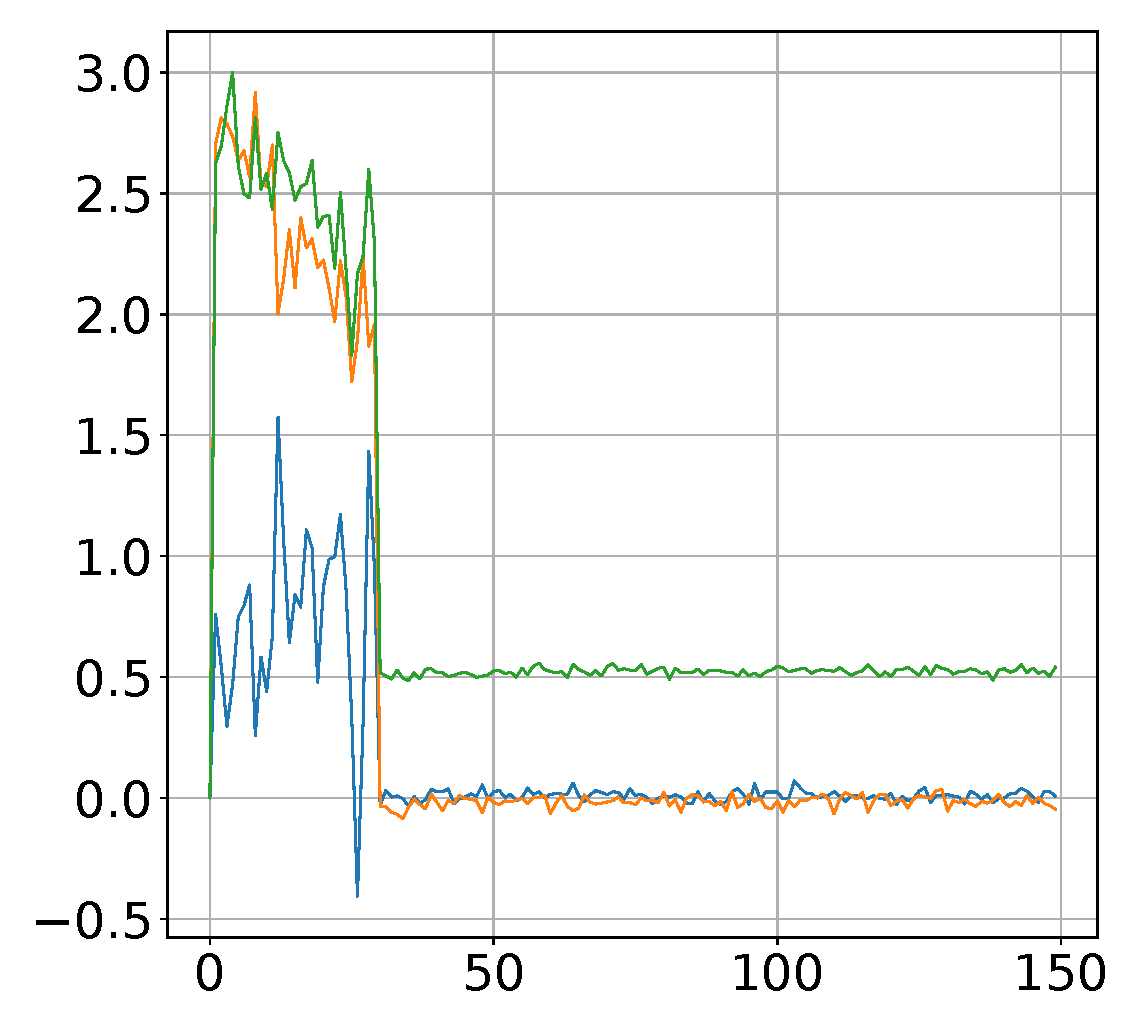
\includegraphics[width = \textwidth]{figures/901noise.eps}
\end{minipage}
\begin{minipage}{.32\textwidth}
\hspace{-2mm}
      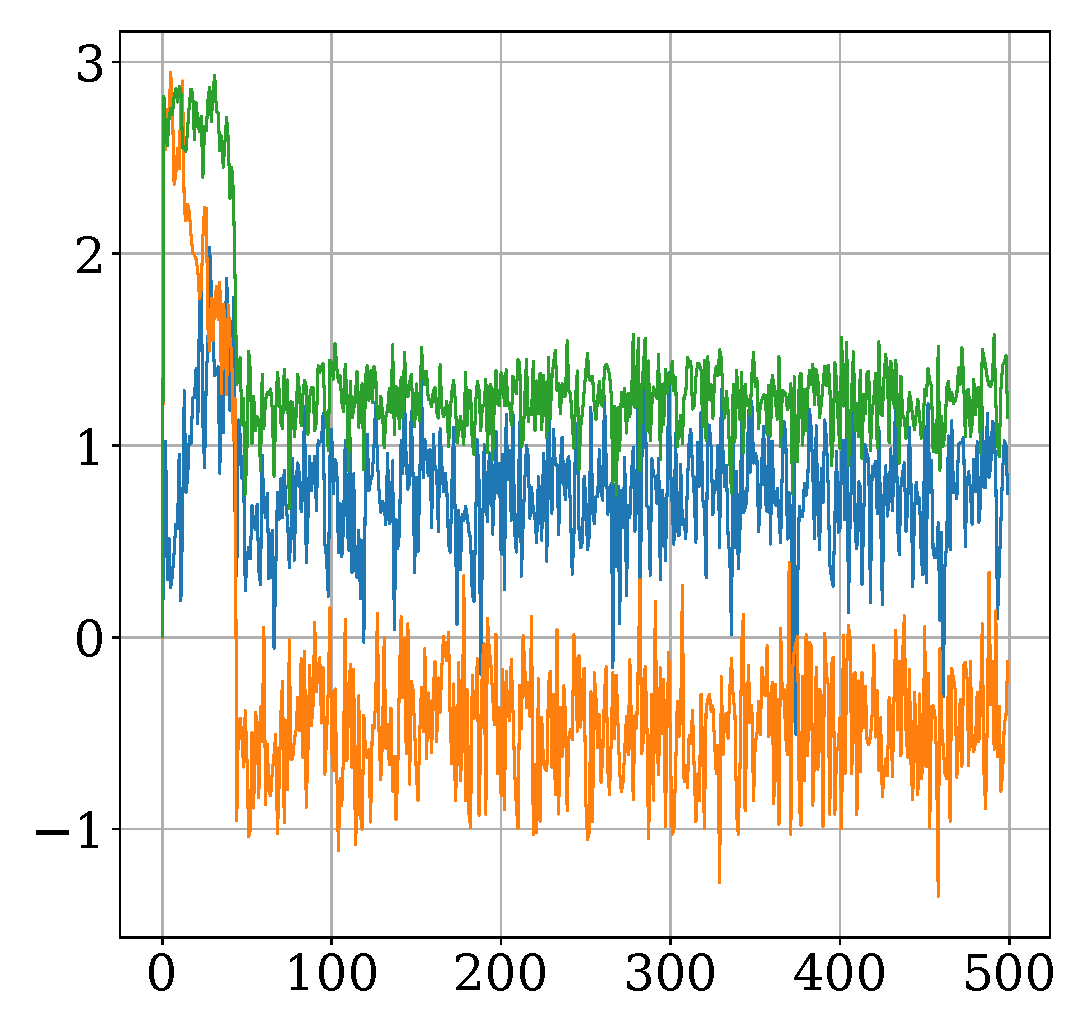
\includegraphics[width = 0.95\textwidth]{figures/902noise.eps}
\end{minipage}
\caption{Зависимость параметров $r$, $x_0$ и $y_0$ от номера итерации при разных априорных распределениях. Сверху вниз: построение с заданием априорного распределения; без задания априорного распределения. Слева на право: окружности без шума; шум в радиусе окружности; шум в радиусе окружности а также произвольные точки по всему изображению.}
\label{ce:fig4}
\end{figure}

В данной части эксперимента показан пример обучения мультимодели для аппроксимации нескольких фигур второго порядка одновременно. В качестве данных используется синтетическая выборка Synthetic~2, которая получена при помощи генерации трех произвольных неперсекающихся окружностей, а также добавления к данным окружностям шума. Шум добавлялся к радиусу окружности для каждой точки, также в выборку были добавлены случайные точки, которые не относятся к окружностям. В эксперименте сравнивается две модели: в первой модели регуляризатор~$R\bigl(\mathbf{V}, \mathbf{W}, E(\Omega)\bigr)=0,$ то есть модель без задания регуляризатора, во второй модели регуляризатор:
\[
R\bigl(\mathbf{V}, \mathbf{W}, E(\Omega)\bigr)= -\sum_{k=1}^{K}\gamma\left(\mathbf{w}_k - \mathbf{w}_k^{0}\right)^{\mathsf{T}}\left(\mathbf{w}_k - \mathbf{w}_k^{0}\right),
\]
где~$\mathbf{w}_k^{0}$ априорные предположения о векторе параметров.

На рис.~\ref{ce:fig3} показан результат построения ансамбля локально аппроксимирующих моделей, которые аппроксимируют выборку. Каждая локальная модель аппроксимирует одну окружность, причем при добавления разного шума, качестве аппроксимации падет.
На рис.~\ref{ce:fig4} показан график зависимости радиуса окружностей $r$ и их центров $(x_0, y_0)$ от номера итерации. Видно, что модель с заданием априорного распределения сходится быстрее чем модель без задания априорного распределения.

\subsection{Эксперимент с разным уровнем шума и дисперсии априорного распределения}
\begin{figure}[h!t]\center
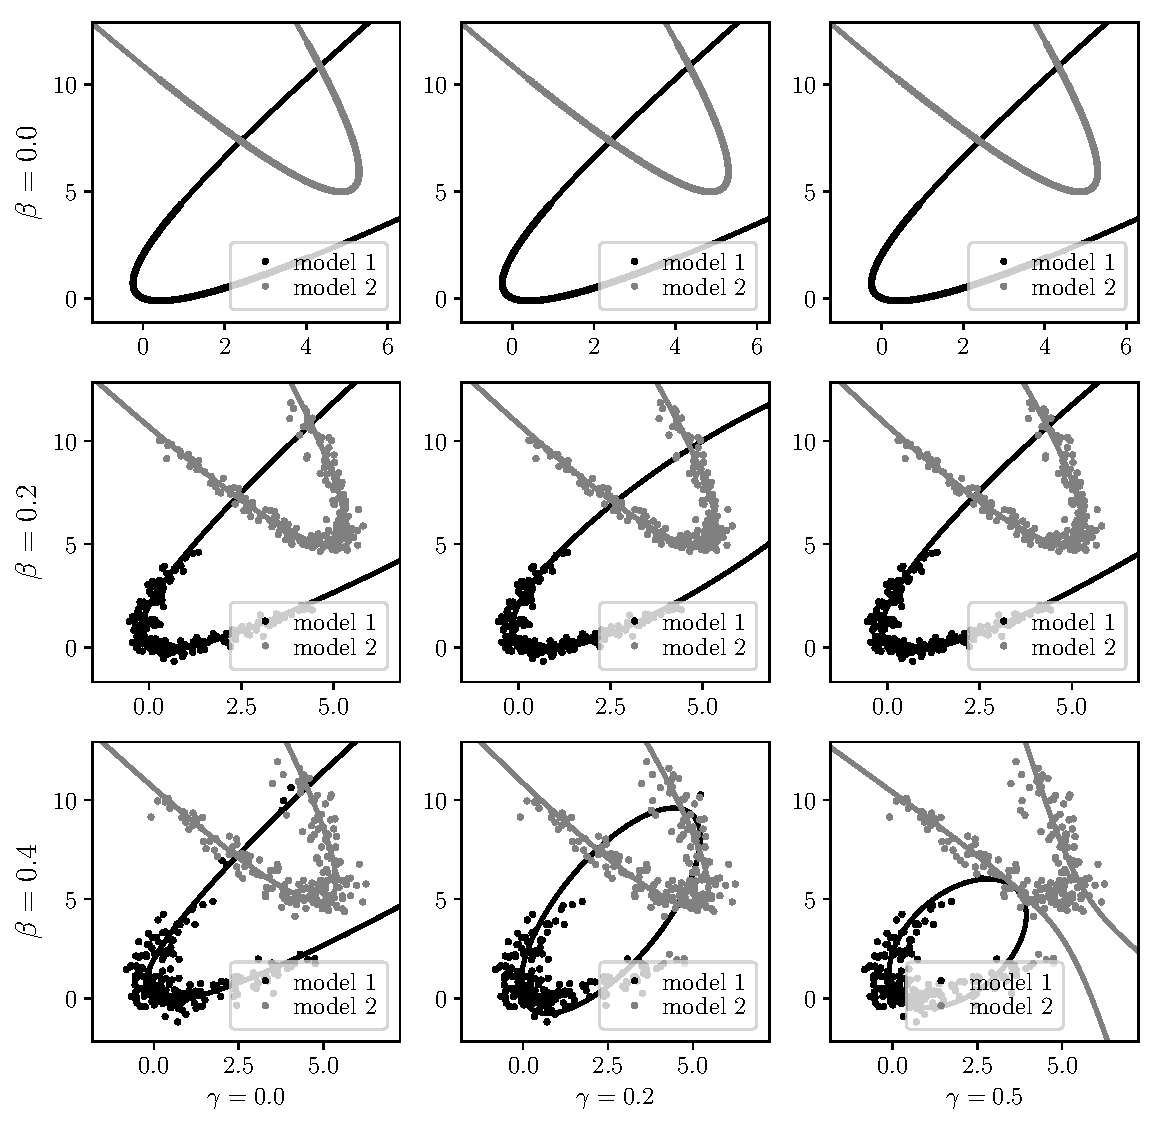
\includegraphics[width=0.8\textwidth]{figures/beta_gamma}
\caption{Результат аппроксимации для данных с разным уровнем шума~$\beta$ и от дисперсии априорного распределения~$\gamma$}
\label{ce:fig6}
\end{figure}

\begin{figure}[h!t]\center
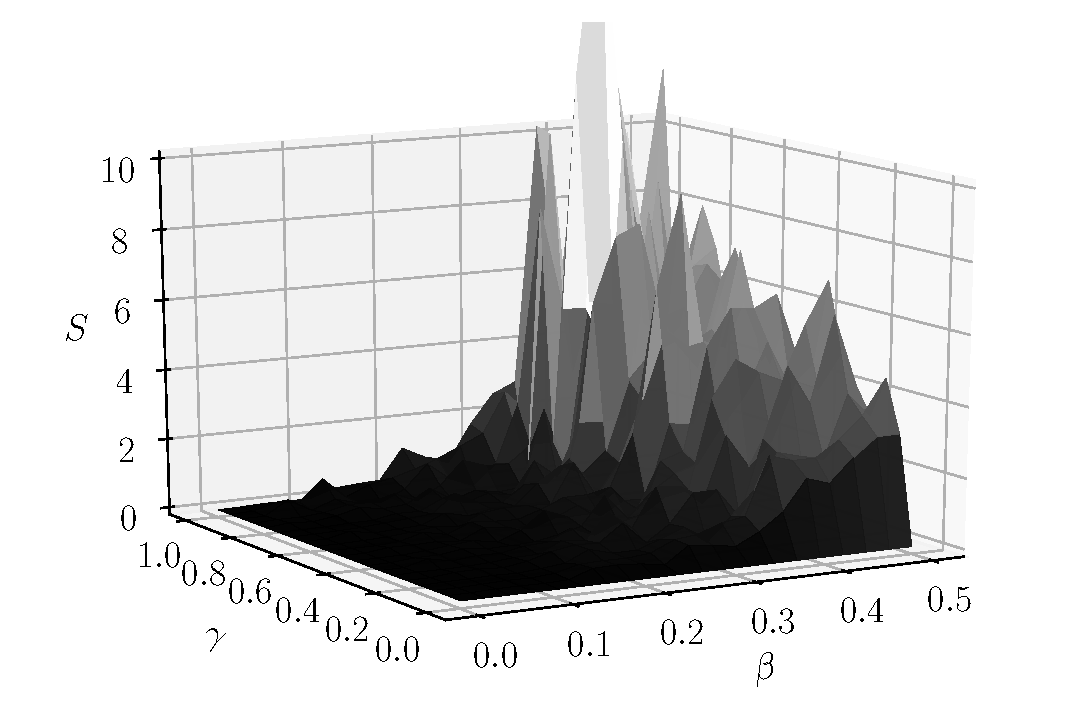
\includegraphics[width=0.5\textwidth]{figures/3dplot}
\caption{Зависимость моделей от уровня шума~$\beta$ в данных, а также от дисперсии априорного распределения~$\gamma$}
\label{ce:fig5}
\end{figure}
В данной части эксперимента проводится анализ качества аппроксимации~$S$ от уровня шума~$\beta$ в данных и от параметра априорных распределений~$\gamma$. Выборка получена следующим образом: сначала случайным образом выбирается два вектора параметров~$\mathbf{w}^{true}_{1}$ и~$\mathbf{w}^{true}_{2}$ --- коэффициенты двух парабол. На основе векторов~$\mathbf{w}^{true}_{1}$ и~$\mathbf{w}^{true}_{2}$ выполняется генерация точек~$x_i$ и~$y_i$ с добавлением нормального шума~$\varepsilon\sim \mathcal{N}\bigr(0, \beta\bigr)$. При обучении мультимодели в качестве априорного распределения параметров рассматривается~$\mathbf{w}_1\sim\mathcal{N}\bigr(\mathbf{w}^{true}_{1}, \gamma\mathbf{I}\bigr),\mathbf{w}_2\sim\mathcal{N}\bigr(\mathbf{w}^{true}_{2}, \gamma\mathbf{I}\bigr)$.

Рассматривается следующий критерий качества:
\[
S = ||\mathbf{w}^{pred}_{1} - \mathbf{w}^{true}_{1}||^{2}_{2} + ||\mathbf{w}^{pred}_{2} - \mathbf{w}^{true}_{2}||^{2}_{2},
\]
где~$\mathbf{w}^{pred}_{1}$ аппроксимация вектора параметров первой локальной модели, а~$\mathbf{w}^{pred}_{2}$ аппроксимация вектора параметров второй локальной модели.

На рис.~\ref{ce:fig5} показана зависимость критерия качества~$S$ от уровня шума~$\beta$ и параметра априорного распределения~$\gamma$. Из графика видно, что при малом уровне шума~$\beta$ качество аппроксимации не зависит от параметра~$\gamma$, а при увеличении шума~$\beta$ качество аппроксимации~$S$ падает.

На рис.~\ref{ce:fig5} показан пример работы алгоритма при разных параметрах~$\beta$ и $\gamma$. Видно, что в случае отсутствия шума~$\beta$ обе локальные модели аппроксимируют выборку. При увеличении уровня шума качество аппроксимации падает: при~$\beta=0{,}2$ при увеличении $\gamma$ первая локальная модель из параболы переходит в эллипс; при~$\beta=0{,}4$ при увеличении  $\gamma$ первая локальная модель из параболы переходит в эллипс, а вторая модель из параболы переходит в гиперболу.



\section{Заключение}
В данной работе проведен анализ смеси экспертов при различных априорных распределениях параметров локальных моделей. В качестве данных использовались кривые второго порядка: парабола, гипербола, эллипс. В качестве шлюзовой функции использовалась двухслойная нейросеть.

В вычислительно эксперименте проведено сравнение сходимости ЕМ--алгоритма при задании априорного распределения и без него. Проведен эксперимент, в котором анализируется качество аппроксимации в зависимости от начального уровня шума в данных, а также в зависимости от параметров регуляризатора. В ходе эксперимента показано, что при увеличении уровня шума в начальных данных, точность аппроксимации падает: при большом шума вид апроксимируемой фигуры изменяется с параболы на гиперболу.


\begin{thebibliography}{99}
\bibitem{Tianqi2016}
	\textit{Chen Tianqi, Guestrin Carlos} XGBoost: A Scalable Tree Boosting System~// KDD ’16 Proceedings of the 22nd ACM SIGKDD International Conference on Knowledge Discovery and Data Mining. 2016.
	
\bibitem{Ishwaran2012}
	\textit{Chen Xi, Ishwaran Hemant} Random Forests for Genomic Data Analysis~// Genomics. 2012. Issues. 99, No 6. pp. 323--329.

\bibitem{Yuksel2012}
	\textit{Yuksel Seniha Esen, Wilson Joseph N., Gader Paul D} Twenty Years of Mixture of Experts~// IEEE Transactions on Neural Networks and Learning Systems. 2012. Issues. 23, No 8. pp. 1177--1193.


\bibitem{Cao2003}
	\textit{L.~Cao} Support vector machines experts for time series forecasting~// Neurocomputing, vol. 51, pp. 321–339, Apr. 2003.

\bibitem{Dempster1977}
	\textit{A. P. Dempster, N. M. Laird and D. B. Rubin} Maximum Likelihood from Incomplete Data via the EM Algorithm~// Journal of the Royal Statistical Society. Series B (Methodological), Vol. 39, No. 1 pp. 1-38, 1977.
	
	
\bibitem{Yumlu2003}
	\textit{M.\,S.~Yumlu, F.\,S.~Gurgen,  N.~Okay} Financial time series prediction using mixture of experts~// in Proc. 18th Int. Symp. Comput. Inf. Sci., 2003, pp. 553--560.
	
\bibitem{Cheung1995}
	\textit{Y.~M.~Cheung, W.~M.~Leung, and L. Xu} Application of mixture of experts model to financial time series forecasting~// in Proc. Int. Conf. Neural Netw. Signal Process., 1995, pp. 1--4.
	
\bibitem{Weigend2000}
	\textit{A. S. Weigend, S. Shi} Predicting daily probability distributions of S\&P500 returns~// J. Forecast., vol. 19, no. 4, pp. 375--392, 2000.
	
\bibitem{Ebrahimpour2009}
	\textit{R. Ebrahimpour, M. R. Moradian, A. Esmkhani, F. M. Jafarlou} Recognition of Persian handwritten digits using characterization loci and mixture of experts~// J. Digital Content Technol. Appl., vol. 3, no. 3, pp. 42–46, 2009.
	
\bibitem{Estabrooks2001}
	\textit{A.~Estabrooks, N.~Japkowicz} A mixture-of-experts framework for text classification~//in Proc. Workshop Comput. Natural Lang. Learn., Assoc. Comput. Linguist., 2001, pp. 1--8.
	
\bibitem{Mossavat2010}
	\textit{S. Mossavat, O. Amft, B. de Vries, P. Petkov, W. Kleijn} A Bayesian hierarchical mixture of experts approach to estimate speech quality~// in Proc. 2nd Int. Workshop Qual. Multimedia Exper., pp. 200--205., 2010
	
\bibitem{Sminchisescu2007}
	\textit{C. Sminchisescu, A. Kanaujia, and D. Metaxas} B M3 E: Discrimina- tive density propagation for visual tracking~// IEEE Trans. Pattern Anal. Mach. Intell., vol. 29, no. 11, pp. 2030–2044, 2007.

	
\bibitem{Matveev2010}
	\textit{I. Matveev} Detection of iris in image by interrelated maxima of brightness gradient projections~// Appl.Comput. Math. 9 (2), 252–257, 2010.

\bibitem{Matveev2014}
	\textit{I. Matveev, I. Simonenko}. Detecting precise iris boundaries by circular shortest path method~// Pattern Recognition and Image Analysis. 24. 304-309. 2014.
	
\bibitem{Bowyer2010}
	\textit{K. Bowyer, K. Hollingsworth, P. Flynn} A Survey of Iris Biometrics Research: 2008–2010.

\bibitem{Peng1996}
	\textit{F. Peng, R. A. Jacobs, M. A. Tanner} Bayesian inference in mixtures-of-experts and hierarchical mixtures-of-experts models with an application to speech recognition~// J. Amer. Stat. Assoc., vol. 91, no. 435, pp. 953–960, 1996.
	
\bibitem{Tuerk2001}
	\textit{A. Tuerk} The state based mixture of experts HMM with applications to the recognition of spontaneous speech~// Ph.D. thesis, Dept. Eng., Univ. Cambridge, Cambridge, U.K., 2001.
	
\bibitem{bishop2006}
	\textit{Bishop C.} Pattern Recognition and Machine Learning.~---~Berlin: Springer, 2006. 758~p.

 \end{thebibliography}


\end{document}

